\documentclass[12pt]{article}
\usepackage[utf8]{inputenc}
\usepackage{amsmath,amsthm,amsfonts,amssymb}
\usepackage{tikz}
% \usepackage{subfig}
\usepackage[english]{babel}
\usepackage{capt-of}
\usepackage{tabularray}
\usepackage{caption}
\usepackage{subcaption}
% \usepackage{subcaption}
% \captionsetup{compatibility=false}
\usepackage{graphicx}
\newtheorem{theorem}{Theorem}
\usetikzlibrary{calc}
\usetikzlibrary{shapes}
\usepackage{hyperref}
%might be unnecessary
\usepackage{doi}

%bibliography CMDS

%\usepackage{cite}
%\usepackage[style=alphabetic]{biblatex}
%\bibliographystyle{plain}

%\usepackage[style=alphabetic]{biblatex}

% \usepackage[backend=biber,style=alphabetic]{biblatex}
\usepackage[backend=biber,style=numeric]{biblatex}
% \usepackage[backend=biber,style=abbrv]{biblatex}
% \usepackage[backend=biber,style=alpha]{biblatex}
%\usepackage[backend=bibtex,style=alphabetic]{biblatex}
\addbibresource{./bibb.bib}

%%% With amsthm package, creates environments for nicely formatted,
%%% labeled, and numbered propositions, etc.
\theoremstyle{plain}

\newtheorem{thm}{Theorem}[section]
\newtheorem{lemma}[thm]{Lemma}
\newtheorem{prop}[thm]{Proposition}
\newtheorem{conj}[thm]{Conjecture}
\newtheorem{cor}[thm]{Corollary}
\newtheorem{claim}[thm]{Claim}
\newtheorem{fact}[thm]{Fact}
\newtheorem{constraint}[thm]{Constraint}

\theoremstyle{definition}
\newtheorem{eg}[thm]{Example}
% \newtheorem{defn}[thm]{Definition}
\newtheorem{definition}{Definition}[section]
\newtheorem{rem}[thm]{Remark}
\newtheorem{observ}[thm]{Observation}
\newtheorem{open}[thm]{Open Problem}
\newtheorem{prob.}[thm]{Problem}
\newtheorem{quest}[thm]{Question}

% I used these for making definitions and theorems, not what is above
\theoremstyle{remark}
\newtheorem{remark}[thm]{Remark}
\newtheorem{note}[thm]{Note}

\theoremstyle{definition}
% \newtheorem{definition}{Definition}[section]
\newtheorem{exmp}{Example}[section]

%custom commands

% blank cell
\newcommand{\cell}[4]{ \draw[thick] ( #1 , #2 ) rectangle ( #3 , #4 );}

% invisible cell for spacing
\newcommand{\spacecell}[4]{ \draw[thick, color=white] ( #1 , #2 ) rectangle ( #3 , #4 );}

% open cell 
\newcommand{\cellopen}[4]{ \draw[thick] ( #1 , #2 ) rectangle ( #3 , #4 ); \node[shape=circle,draw=red,fill=red, inner sep=0pt,minimum size=3pt] (A) at ( #1 * 0.5 + #3 * 0.5 , #2 * 0.5 + #4 * 0.5 ){};}
% /
% \newcommand{\cellA}[4]{ \draw[thick] ( #1 , #2 ) rectangle ( #3 , #4 ); \draw[red, thick, densely dotted] (#3 * 0.5 + #1 * 0.5 , #2) -- (#3, #4 * 0.5 + #2 * 0.5);}
% \
% \newcommand{\cellB}[4]{ \draw[thick] ( #1 , #2 ) rectangle ( #3 , #4 ); \draw[red, thick, densely dotted] (#3 * 0.5 + #1 * 0.5 , #2) -- (#1, #4 * 0.5 + #2 * 0.5);}
% /
% \newcommand{\cellC}[4]{ \draw[thick] ( #1 , #2 ) rectangle ( #3 , #4 ); \draw[red, thick, densely dotted] (#3 * 0.5 + #1 * 0.5 , #4) -- (#1, #4 * 0.5 + #2 * 0.5);}
% L
% \newcommand{\cellD}[4]{ \draw[thick] ( #1 , #2 ) rectangle ( #3 , #4 ); \draw[red, thick, densely dotted] (#3 * 0.5 + #1 * 0.5 , #4) -- (#3, #4 * 0.5 + #2 * 0.5);}
% |
% \newcommand{\cellE}[4]{ \draw[thick] ( #1 , #2 ) rectangle ( #3 , #4 ); \draw[red, thick, densely dotted] (#3 * 0.5 + #1 * 0.5 , #2) -- (#3 * 0.5 + #1 * 0.5 , #4);}
% % -
% \newcommand{\cellF}[4]{ \draw[thick] ( #1 , #2 ) rectangle ( #3 , #4 ); \draw[red, thick, densely dotted] (#3, #4 * 0.5 + #2 * 0.5) -- (#1, #4 * 0.5 + #2 * 0.5);}

% \newcommand{\cellAf}[4]{\filldraw[gray!40] ( #1 , #2 ) rectangle ( #3 , #4 ); \draw[thick] ( #1 , #2 ) rectangle ( #3 , #4 ); \draw[red, thick, densely dotted] (#3 * 0.5 + #1 * 0.5 , #2) -- (#3, #4 * 0.5 + #2 * 0.5);}
% \
% \newcommand{\cellBf}[4]{\filldraw[gray!40] ( #1 , #2 ) rectangle ( #3 , #4 ); \draw[thick] ( #1 , #2 ) rectangle ( #3 , #4 ); \draw[red, thick, densely dotted] (#3 * 0.5 + #1 * 0.5 , #2) -- (#1, #4 * 0.5 + #2 * 0.5);}
% /
% \newcommand{\cellCf}[4]{\filldraw[gray!40] ( #1 , #2 ) rectangle ( #3 , #4 ); \draw[thick] ( #1 , #2 ) rectangle ( #3 , #4 ); \draw[red, thick, densely dotted] (#3 * 0.5 + #1 * 0.5 , #4) -- (#1, #4 * 0.5 + #2 * 0.5);}
% L
% \newcommand{\cellDf}[4]{\filldraw[gray!40] ( #1 , #2 ) rectangle ( #3 , #4 ); \draw[thick] ( #1 , #2 ) rectangle ( #3 , #4 ); \draw[red, thick, densely dotted] (#3 * 0.5 + #1 * 0.5 , #4) -- (#3, #4 * 0.5 + #2 * 0.5);}
% |
% \newcommand{\cellEf}[4]{\filldraw[gray!40] ( #1 , #2 ) rectangle ( #3 , #4 ); \draw[thick] ( #1 , #2 ) rectangle ( #3 , #4 ); \draw[red, thick, densely dotted] (#3 * 0.5 + #1 * 0.5 , #2) -- (#3 * 0.5 + #1 * 0.5 , #4);}
% % -
% \newcommand{\cellFf}[4]{\filldraw[gray!40] ( #1 , #2 ) rectangle ( #3 , #4 ); \draw[thick] ( #1 , #2 ) rectangle ( #3 , #4 ); \draw[red, thick, densely dotted] (#3, #4 * 0.5 + #2 * 0.5) -- (#1, #4 * 0.5 + #2 * 0.5);}


\newcommand{\cellA}[4]{\draw[red, thick, densely dotted] ( #1 + 0.5 , #2 ) arc(0:90:{0.5}); \draw[thick] ( #1 , #2 ) rectangle ( #3 , #4 );}
\newcommand{\cellB}[4]{\draw[red, thick, densely dotted] ( #1 + 1 , #2 + 0.5 ) arc(90:180:{0.5}); \draw[thick] ( #1 , #2 ) rectangle ( #3 , #4 );}
\newcommand{\cellC}[4]{\draw[red, thick, densely dotted] ( #1 + 0.5, #2 + 1 ) arc(180:270:{0.5}); \draw[thick] ( #1 , #2 ) rectangle ( #3 , #4 );}
\newcommand{\cellD}[4]{\draw[red, thick, densely dotted] ( #1 , #2 + 0.5 ) arc(-90:0:{0.5}); \draw[thick] ( #1 , #2 ) rectangle ( #3 , #4 );}
\newcommand{\cellE}[4]{\draw[red, thick, densely dotted] (#3, #4 * 0.5 + #2 * 0.5) -- (#1, #4 * 0.5 + #2 * 0.5); \draw[thick] ( #1 , #2 ) rectangle ( #3 , #4 );}
\newcommand{\cellF}[4]{\draw[red, thick, densely dotted] (#3 * 0.5 + #1 * 0.5 , #2) -- (#3 * 0.5 + #1 * 0.5 , #4); \draw[thick] ( #1 , #2 ) rectangle ( #3 , #4 );}
\newcommand{\cellG}[4]{\draw[red, thick, densely dotted] ( #1 + 0.5 , #2 ) arc(0:90:{0.5}); \draw[red, thick, densely dotted] ( #1 + 0.5, #2 + 1 ) arc(180:270:{0.5}); \draw[thick] ( #1 , #2 ) rectangle ( #3 , #4 );}
\newcommand{\cellH}[4]{\draw[red, thick, densely dotted] ( #1 , #2 + 0.5 ) arc(-90:0:{0.5}); \draw[red, thick, densely dotted] ( #1 + 1 , #2 + 0.5 ) arc(90:180:{0.5}); \draw[thick] ( #1 , #2 ) rectangle ( #3 , #4 );}
\newcommand{\cellI}[4]{\draw[red, thick, densely dotted] (#3 * 0.5 + #1 * 0.5 , #2) -- (#3 * 0.5 + #1 * 0.5 , #4); \node[shape=circle,draw=none,fill=white, inner sep=3pt,minimum size=5pt] (A) at ( #1 + 0.5 , #2 + 0.5 ) {}; \draw[red, thick, densely dotted] (#3, #4 * 0.5 + #2 * 0.5) -- (#1, #4 * 0.5 + #2 * 0.5); \draw[thick] ( #1 , #2 ) rectangle ( #3 , #4 );}
\newcommand{\cellJ}[4]{\draw[red, thick, densely dotted] (#3, #4 * 0.5 + #2 * 0.5) -- (#1, #4 * 0.5 + #2 * 0.5); \node[shape=circle,draw=none,fill=white, inner sep=3pt,minimum size=5pt] (A) at ( #1 + 0.5 , #2 + 0.5 ) {}; \draw[thick] ( #1 , #2 ) rectangle ( #3 , #4 ); \draw[red, thick, densely dotted] (#3 * 0.5 + #1 * 0.5 , #2) -- (#3 * 0.5 + #1 * 0.5 , #4);}


\newcommand{\cellAf}[4]{\filldraw[gray!40] ( #1 , #2 ) rectangle ( #3 , #4 ); \draw[red, thick, densely dotted] ( #1 + 0.5 , #2 ) arc(0:90:{0.5}); \draw[thick] ( #1 , #2 ) rectangle ( #3 , #4 );}
\newcommand{\cellBf}[4]{\filldraw[gray!40] ( #1 , #2 ) rectangle ( #3 , #4 ); \draw[red, thick, densely dotted] ( #1 + 1 , #2 + 0.5 ) arc(90:180:{0.5}); \draw[thick] ( #1 , #2 ) rectangle ( #3 , #4 );}
\newcommand{\cellCf}[4]{\filldraw[gray!40] ( #1 , #2 ) rectangle ( #3 , #4 ); \draw[red, thick, densely dotted] ( #1 + 0.5, #2 + 1 ) arc(180:270:{0.5}); \draw[thick] ( #1 , #2 ) rectangle ( #3 , #4 );}
\newcommand{\cellDf}[4]{\filldraw[gray!40] ( #1 , #2 ) rectangle ( #3 , #4 ); \draw[red, thick, densely dotted] ( #1 , #2 + 0.5 ) arc(-90:0:{0.5}); \draw[thick] ( #1 , #2 ) rectangle ( #3 , #4 );}
\newcommand{\cellEf}[4]{\filldraw[gray!40] ( #1 , #2 ) rectangle ( #3 , #4 ); \draw[red, thick, densely dotted] (#3, #4 * 0.5 + #2 * 0.5) -- (#1, #4 * 0.5 + #2 * 0.5); \draw[thick] ( #1 , #2 ) rectangle ( #3 , #4 );}
\newcommand{\cellFf}[4]{\filldraw[gray!40] ( #1 , #2 ) rectangle ( #3 , #4 ); \draw[red, thick, densely dotted] (#3 * 0.5 + #1 * 0.5 , #2) -- (#3 * 0.5 + #1 * 0.5 , #4); \draw[thick] ( #1 , #2 ) rectangle ( #3 , #4 );}
\newcommand{\cellGf}[4]{\filldraw[gray!40] ( #1 , #2 ) rectangle ( #3 , #4 ); \draw[red, thick, densely dotted] ( #1 + 0.5 , #2 ) arc(0:90:{0.5}); \draw[red, thick, densely dotted] ( #1 + 0.5, #2 + 1 ) arc(180:270:{0.5}); \draw[thick] ( #1 , #2 ) rectangle ( #3 , #4 );}
\newcommand{\cellHf}[4]{\filldraw[gray!40] ( #1 , #2 ) rectangle ( #3 , #4 ); \draw[red, thick, densely dotted] ( #1 , #2 + 0.5 ) arc(-90:0:{0.5}); \draw[red, thick, densely dotted] ( #1 + 1 , #2 + 0.5 ) arc(90:180:{0.5}); \draw[thick] ( #1 , #2 ) rectangle ( #3 , #4 );}
\newcommand{\cellIf}[4]{\filldraw[gray!40] ( #1 , #2 ) rectangle ( #3 , #4 ); \draw[red, thick, densely dotted] (#3 * 0.5 + #1 * 0.5 , #2) -- (#3 * 0.5 + #1 * 0.5 , #4); \node[shape=circle,draw=none,fill=gray!40, inner sep=3pt,minimum size=5pt] (A) at ( #1 + 0.5 , #2 + 0.5 ) {}; \draw[red, thick, densely dotted] (#3, #4 * 0.5 + #2 * 0.5) -- (#1, #4 * 0.5 + #2 * 0.5); \draw[thick] ( #1 , #2 ) rectangle ( #3 , #4 );}
\newcommand{\cellJf}[4]{\filldraw[gray!40] ( #1 , #2 ) rectangle ( #3 , #4 ); \draw[red, thick, densely dotted] (#3, #4 * 0.5 + #2 * 0.5) -- (#1, #4 * 0.5 + #2 * 0.5); \node[shape=circle,draw=none,fill=gray!40, inner sep=3pt,minimum size=5pt] (A) at ( #1 + 0.5 , #2 + 0.5 ) {}; \draw[thick] ( #1 , #2 ) rectangle ( #3 , #4 ); \draw[red, thick, densely dotted] (#3 * 0.5 + #1 * 0.5 , #2) -- (#3 * 0.5 + #1 * 0.5 , #4);}


\newcommand{\lablnode}[3]{\node[shape=circle,draw=none,fill=none, inner sep=0pt,minimum size=5pt] (A) at ( #1 , #2 ) {#3};}
\newcommand{\lablvertex}[3]{\node[shape=circle,draw=none,fill=white, inner sep=2pt,minimum size=5pt] (A) at ( #1 , #2 ) {#3};}

%doc info
\title{Mosaics}
\author{Jack Hanke}
\date{\today}

\begin{document}

\begin{center}
    \Large
    \textbf{Mosaics}
    
    \vspace{0.4cm}
    \large
    
    Jack Hanke   
    \vspace{0.4cm}
    
    \today
    \vspace{0.4cm}    
\end{center}

\section{THIS IS NEW}



It is useful to define an index for vertex labelings of these $m \times 1$ columns. To do this, consider reading a column of vertex labelings from bottom to top, ignoring the first and last $0$'s. If we interpret these sequences for the left and right column as binary numbers $b_{left}$ and $b_{right}$, the index in base ten is the pair $(b_{left}, b_{right})$. For example, for the above $m=3$ column, we have sequences $00$ for the left column and $10$ for the right column, so the index is $(0,2)$.

Next consider a column with index $(0, b_{1})$ for some $b_{1} \in [0,2^{m-1}-1]$. For reasons we will see later, let's call this the \textit{starting column}. Now consider appending a column with index $(b_{1}, b_{2})$ for some $b_{2} \in [0,2^{m-1}-1]$. For example, below is a diagram for appending our starting column $(0,2)$ with column $(2,3)$. 

\begin{center}
    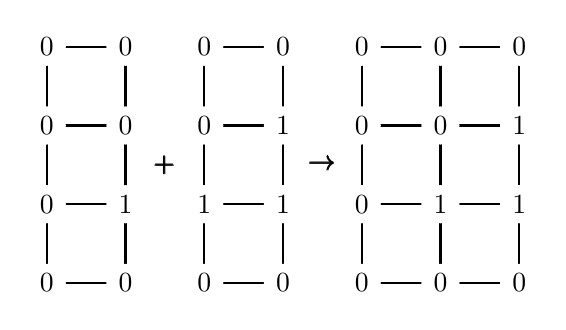
\begin{tikzpicture}
        \cell{0}{0}{1}{1}
        \cell{0}{1}{1}{2}
        \cell{0}{2}{1}{3}
        % col 1
        \( \lablvertex{0}{0}{$0$} \)
        \( \lablvertex{0}{1}{$0$} \)
        \( \lablvertex{0}{2}{$0$} \)
        \( \lablvertex{0}{3}{$0$} \)
        % col 2
        \( \lablvertex{1}{0}{$0$} \)
        \( \lablvertex{1}{1}{$1$} \)
        \( \lablvertex{1}{2}{$0$} \)
        \( \lablvertex{1}{3}{$0$} \)

        % plus
        \( \lablnode{1.5}{1.5}{$\pmb{+}$} \)

        \cell{2}{0}{3}{1}
        \cell{2}{1}{3}{2}
        \cell{2}{2}{3}{3}
        % col 1
        \( \lablvertex{2}{0}{$0$} \)
        \( \lablvertex{2}{1}{$1$} \)
        \( \lablvertex{2}{2}{$0$} \)
        \( \lablvertex{2}{3}{$0$} \)
        % col 1
        \( \lablvertex{3}{0}{$0$} \)
        \( \lablvertex{3}{1}{$1$} \)
        \( \lablvertex{3}{2}{$1$} \)
        \( \lablvertex{3}{3}{$0$} \)

        \( \lablnode{3.5}{1.5}{$\pmb{\to}$} \)

        \cell{4}{0}{5}{1}
        \cell{4}{1}{5}{2}
        \cell{4}{2}{5}{3}
        \cell{5}{0}{6}{1}
        \cell{5}{1}{6}{2}
        \cell{5}{2}{6}{3}

        % col 1
        \( \lablvertex{4}{0}{$0$} \)
        \( \lablvertex{4}{1}{$0$} \)
        \( \lablvertex{4}{2}{$0$} \)
        \( \lablvertex{4}{3}{$0$} \)
        % col 2
        \( \lablvertex{5}{0}{$0$} \)
        \( \lablvertex{5}{1}{$1$} \)
        \( \lablvertex{5}{2}{$0$} \)
        \( \lablvertex{5}{3}{$0$} \)
        % col 3
        \( \lablvertex{6}{0}{$0$} \)
        \( \lablvertex{6}{1}{$1$} \)
        \( \lablvertex{6}{2}{$1$} \)
        \( \lablvertex{6}{3}{$0$} \)


    \end{tikzpicture}
\end{center}

Notice that in the above example we have created a vertex labeling for an $m \times 2$ grid of cells, in which the left-most vertex column labels are all $0$ (left index of $0$). Also note that we did not create either illegal cell labelings with column $(2,3)$. However, we could append the column $(2,1)$, which would create an illegal cell labeling. 

Finally, if we further appended a column with label $(b_2,0)$, we would have created a vertex labeling with a boundary of all $0$'s. For this reason, let's call a column with index $(b,0)$ for $b \in [0,2^{m-1}-1]$ an \textit{ending column}. This vertex labeling would correspond with $1$ polygon mosaic if the middle column had index $(2,3)$, but not if the middle column had index $(2,1)$.

This motivates the creation of a matrix $A(m)$ to every column index $(i,j)$, where $A(m)_{i,j}=1$ if the column labeling corresponds with a legal polygon mosaic, and $0$ otherwise. For example, the $A(3)$ matrix corresponds with the following labeled columns. 

\begin{center}
    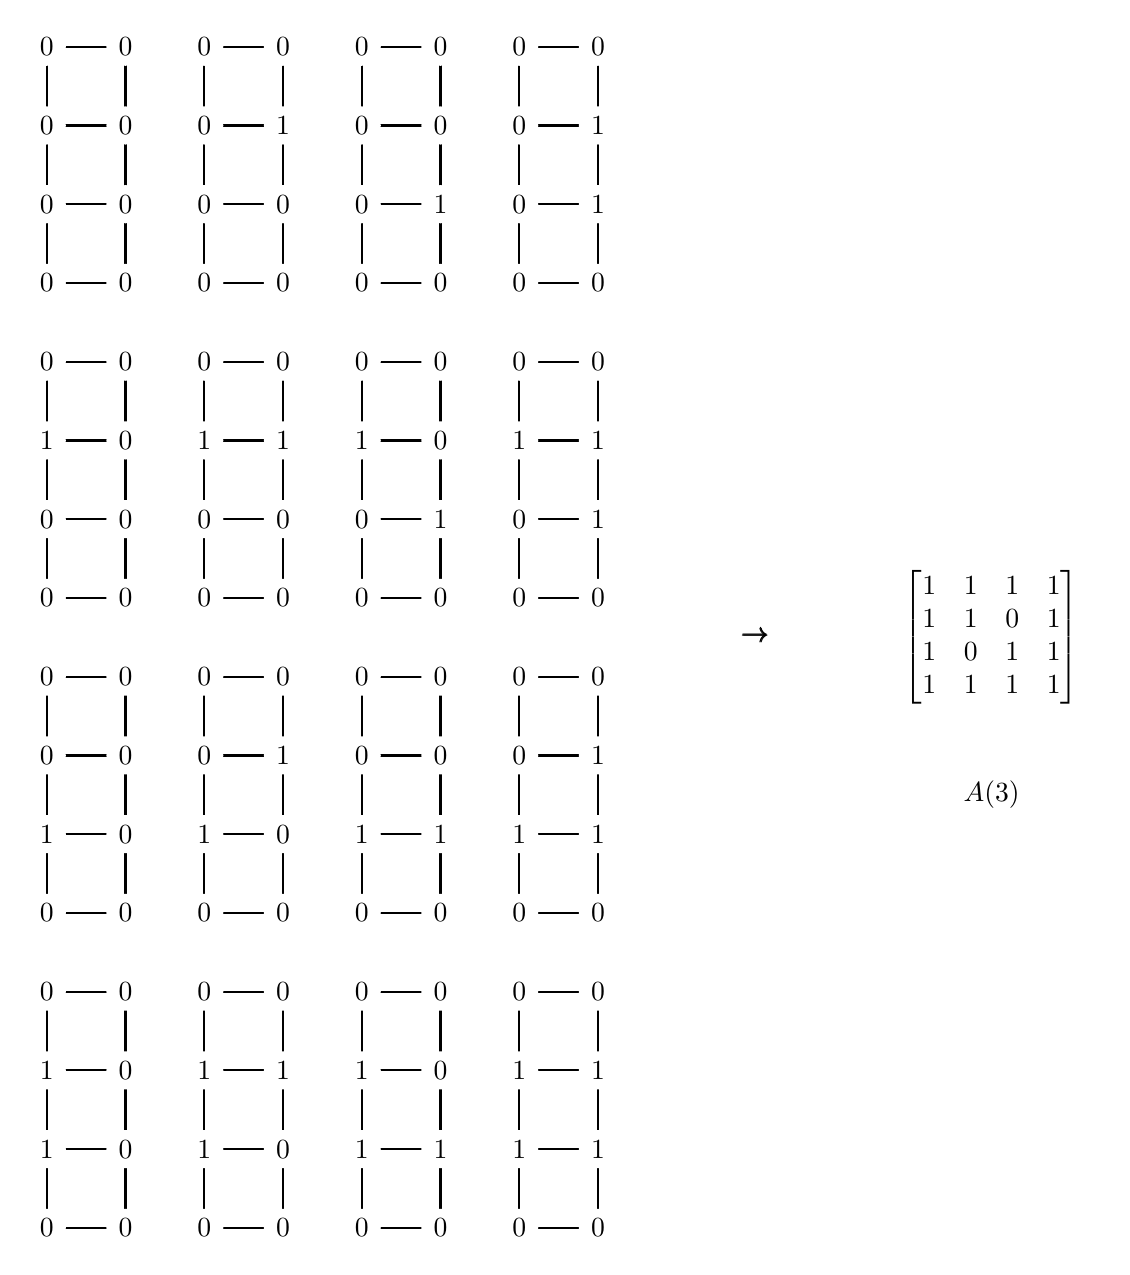
\begin{tikzpicture}
        % row1
        \cell{0}{0}{1}{1}
        \cell{0}{1}{1}{2}
        \cell{0}{2}{1}{3}

        \cell{2}{0}{3}{1}
        \cell{2}{1}{3}{2}
        \cell{2}{2}{3}{3}

        \cell{4}{0}{5}{1}
        \cell{4}{1}{5}{2}
        \cell{4}{2}{5}{3}

        \cell{6}{0}{7}{1}
        \cell{6}{1}{7}{2}
        \cell{6}{2}{7}{3}
        % row2
        \cell{0}{4}{1}{5}
        \cell{0}{5}{1}{6}
        \cell{0}{6}{1}{7}

        \cell{2}{4}{3}{5}
        \cell{2}{5}{3}{6}
        \cell{2}{6}{3}{7}

        \cell{4}{4}{5}{5}
        \cell{4}{5}{5}{6}
        \cell{4}{6}{5}{7}

        \cell{6}{4}{7}{5}
        \cell{6}{5}{7}{6}
        \cell{6}{6}{7}{7}
        % row3
        \cell{0}{8}{1}{9}
        \cell{0}{9}{1}{10}
        \cell{0}{10}{1}{11}

        \cell{2}{8}{3}{9}
        \cell{2}{9}{3}{10}
        \cell{2}{10}{3}{11}

        \cell{4}{8}{5}{9}
        \cell{4}{9}{5}{10}
        \cell{4}{10}{5}{11}

        \cell{6}{8}{7}{9}
        \cell{6}{9}{7}{10}
        \cell{6}{10}{7}{11}
        % row4
        \cell{0}{12}{1}{13}
        \cell{0}{13}{1}{14}
        \cell{0}{14}{1}{15}

        \cell{2}{12}{3}{13}
        \cell{2}{13}{3}{14}
        \cell{2}{14}{3}{15}

        \cell{4}{12}{5}{13}
        \cell{4}{13}{5}{14}
        \cell{4}{14}{5}{15}

        \cell{6}{12}{7}{13}
        \cell{6}{13}{7}{14}
        \cell{6}{14}{7}{15}
        % row 1
        \( \lablvertex{0}{0}{$0$} \)
        \( \lablvertex{0}{1}{$1$} \)
        \( \lablvertex{0}{2}{$1$} \)
        \( \lablvertex{0}{3}{$0$} \)
        
        \( \lablvertex{1}{0}{$0$} \)
        \( \lablvertex{1}{1}{$0$} \)
        \( \lablvertex{1}{2}{$0$} \)
        \( \lablvertex{1}{3}{$0$} \)
        
        \( \lablvertex{2}{0}{$0$} \)
        \( \lablvertex{2}{1}{$1$} \)
        \( \lablvertex{2}{2}{$1$} \)
        \( \lablvertex{2}{3}{$0$} \)
        
        \( \lablvertex{3}{0}{$0$} \)
        \( \lablvertex{3}{1}{$0$} \)
        \( \lablvertex{3}{2}{$1$} \)
        \( \lablvertex{3}{3}{$0$} \)
        
        \( \lablvertex{4}{0}{$0$} \)
        \( \lablvertex{4}{1}{$1$} \)
        \( \lablvertex{4}{2}{$1$} \)
        \( \lablvertex{4}{3}{$0$} \)
        
        \( \lablvertex{5}{0}{$0$} \)
        \( \lablvertex{5}{1}{$1$} \)
        \( \lablvertex{5}{2}{$0$} \)
        \( \lablvertex{5}{3}{$0$} \)
        
        \( \lablvertex{6}{0}{$0$} \)
        \( \lablvertex{6}{1}{$1$} \)
        \( \lablvertex{6}{2}{$1$} \)
        \( \lablvertex{6}{3}{$0$} \)
        
        \( \lablvertex{7}{0}{$0$} \)
        \( \lablvertex{7}{1}{$1$} \)
        \( \lablvertex{7}{2}{$1$} \)
        \( \lablvertex{7}{3}{$0$} \)
        % row 2
        \( \lablvertex{0}{4}{$0$} \)
        \( \lablvertex{0}{5}{$1$} \)
        \( \lablvertex{0}{6}{$0$} \)
        \( \lablvertex{0}{7}{$0$} \)
        
        \( \lablvertex{1}{4}{$0$} \)
        \( \lablvertex{1}{5}{$0$} \)
        \( \lablvertex{1}{6}{$0$} \)
        \( \lablvertex{1}{7}{$0$} \)
        
        \( \lablvertex{2}{4}{$0$} \)
        \( \lablvertex{2}{5}{$1$} \)
        \( \lablvertex{2}{6}{$0$} \)
        \( \lablvertex{2}{7}{$0$} \)
        
        \( \lablvertex{3}{4}{$0$} \)
        \( \lablvertex{3}{5}{$0$} \)
        \( \lablvertex{3}{6}{$1$} \)
        \( \lablvertex{3}{7}{$0$} \)
        
        \( \lablvertex{4}{4}{$0$} \)
        \( \lablvertex{4}{5}{$1$} \)
        \( \lablvertex{4}{6}{$0$} \)
        \( \lablvertex{4}{7}{$0$} \)
        
        \( \lablvertex{5}{4}{$0$} \)
        \( \lablvertex{5}{5}{$1$} \)
        \( \lablvertex{5}{6}{$0$} \)
        \( \lablvertex{5}{7}{$0$} \)
        
        \( \lablvertex{6}{4}{$0$} \)
        \( \lablvertex{6}{5}{$1$} \)
        \( \lablvertex{6}{6}{$0$} \)
        \( \lablvertex{6}{7}{$0$} \)
        
        \( \lablvertex{7}{4}{$0$} \)
        \( \lablvertex{7}{5}{$1$} \)
        \( \lablvertex{7}{6}{$1$} \)
        \( \lablvertex{7}{7}{$0$} \)
        % row 3
        \( \lablvertex{0}{8}{$0$} \)
        \( \lablvertex{0}{9}{$0$} \)
        \( \lablvertex{0}{10}{$1$} \)
        \( \lablvertex{0}{11}{$0$} \)
        
        \( \lablvertex{1}{8}{$0$} \)
        \( \lablvertex{1}{9}{$0$} \)
        \( \lablvertex{1}{10}{$0$} \)
        \( \lablvertex{1}{11}{$0$} \)
        
        \( \lablvertex{2}{8}{$0$} \)
        \( \lablvertex{2}{9}{$0$} \)
        \( \lablvertex{2}{10}{$1$} \)
        \( \lablvertex{2}{11}{$0$} \)
        
        \( \lablvertex{3}{8}{$0$} \)
        \( \lablvertex{3}{9}{$0$} \)
        \( \lablvertex{3}{10}{$1$} \)
        \( \lablvertex{3}{11}{$0$} \)
        
        \( \lablvertex{4}{8}{$0$} \)
        \( \lablvertex{4}{9}{$0$} \)
        \( \lablvertex{4}{10}{$1$} \)
        \( \lablvertex{4}{11}{$0$} \)
        
        \( \lablvertex{5}{8}{$0$} \)
        \( \lablvertex{5}{9}{$1$} \)
        \( \lablvertex{5}{10}{$0$} \)
        \( \lablvertex{5}{11}{$0$} \)
        
        \( \lablvertex{6}{8}{$0$} \)
        \( \lablvertex{6}{9}{$0$} \)
        \( \lablvertex{6}{10}{$1$} \)
        \( \lablvertex{6}{11}{$0$} \)
        
        \( \lablvertex{7}{8}{$0$} \)
        \( \lablvertex{7}{9}{$1$} \)
        \( \lablvertex{7}{10}{$1$} \)
        \( \lablvertex{7}{11}{$0$} \)
        % row 4
        \( \lablvertex{0}{12}{$0$} \)
        \( \lablvertex{0}{13}{$0$} \)
        \( \lablvertex{0}{14}{$0$} \)
        \( \lablvertex{0}{15}{$0$} \)
        
        \( \lablvertex{1}{12}{$0$} \)
        \( \lablvertex{1}{13}{$0$} \)
        \( \lablvertex{1}{14}{$0$} \)
        \( \lablvertex{1}{15}{$0$} \)
        
        \( \lablvertex{2}{12}{$0$} \)
        \( \lablvertex{2}{13}{$0$} \)
        \( \lablvertex{2}{14}{$0$} \)
        \( \lablvertex{2}{15}{$0$} \)
        
        \( \lablvertex{3}{12}{$0$} \)
        \( \lablvertex{3}{13}{$0$} \)
        \( \lablvertex{3}{14}{$1$} \)
        \( \lablvertex{3}{15}{$0$} \)
        
        \( \lablvertex{4}{12}{$0$} \)
        \( \lablvertex{4}{13}{$0$} \)
        \( \lablvertex{4}{14}{$0$} \)
        \( \lablvertex{4}{15}{$0$} \)
        
        \( \lablvertex{5}{12}{$0$} \)
        \( \lablvertex{5}{13}{$1$} \)
        \( \lablvertex{5}{14}{$0$} \)
        \( \lablvertex{5}{15}{$0$} \)
        
        \( \lablvertex{6}{12}{$0$} \)
        \( \lablvertex{6}{13}{$0$} \)
        \( \lablvertex{6}{14}{$0$} \)
        \( \lablvertex{6}{15}{$0$} \)
        
        \( \lablvertex{7}{12}{$0$} \)
        \( \lablvertex{7}{13}{$1$} \)
        \( \lablvertex{7}{14}{$1$} \)
        \( \lablvertex{7}{15}{$0$} \)

        % arrow
        \( \lablnode{9}{7.5}{$\pmb{\to}$} \)
        % matrix
        \( \lablnode{12}{7.5}{$\begin{bmatrix} 1 & 1 & 1 & 1 \\ 1 & 1 & 0 & 1 \\ 1 & 0 & 1 & 1 \\ 1 & 1 & 1 & 1 \end{bmatrix}$} \)

        \( \lablnode{12}{5.5}{$A(3)$} \)

    \end{tikzpicture}
\end{center}

$A(m)$ has the property that the $0$-th row represets all starting columns, and the $0$-th column represents all ending columns. Even more importantly, notice that $A(m)^2_{i,j}$ represents the number of $m \times 2$ grids with left-most index $i$ and right-most index $j$ that correspond with a legal polygon mosaic. In general, $(A(m)^n)_{i,j}$ represents this quantity for an $m \times n$ grid of cells, and so if we know $A(m)$ for some $m$, then $(A(m)^n)_{0,0} = p_{m,n}.$

The final component of the proof is constructing $A(m)$ for any $m$. Begin by  calculating $A(2)$ by identifying the number of legal polygon mosaics that correspond with each vertex coloring index $\{(0,0),(0,1),(1,0),(1,1)\}$, like so.

\begin{center}
    \begin{tikzpicture}
        % row1
        \cell{0}{0}{1}{1}
        \cell{0}{1}{1}{2}
        
        \cell{2}{0}{3}{1}
        \cell{2}{1}{3}{2}
        
        % row2
        \cell{0}{3}{1}{4}
        \cell{0}{4}{1}{5}
        
        \cell{2}{3}{3}{4}
        \cell{2}{4}{3}{5}
        % row 1
        \( \lablvertex{0}{0}{$0$} \)
        \( \lablvertex{0}{1}{$1$} \)
        \( \lablvertex{0}{2}{$0$} \)
        
        \( \lablvertex{1}{0}{$0$} \)
        \( \lablvertex{1}{1}{$0$} \)
        \( \lablvertex{1}{2}{$0$} \)
        
        \( \lablvertex{2}{0}{$0$} \)
        \( \lablvertex{2}{1}{$1$} \)
        \( \lablvertex{2}{2}{$0$} \)
        
        \( \lablvertex{3}{0}{$0$} \)
        \( \lablvertex{3}{1}{$1$} \)
        \( \lablvertex{3}{2}{$0$} \)
        % row 2
        \( \lablvertex{0}{3}{$0$} \)
        \( \lablvertex{0}{4}{$0$} \)
        \( \lablvertex{0}{5}{$0$} \)
        
        \( \lablvertex{1}{3}{$0$} \)
        \( \lablvertex{1}{4}{$0$} \)
        \( \lablvertex{1}{5}{$0$} \)
        
        \( \lablvertex{2}{3}{$0$} \)
        \( \lablvertex{2}{4}{$0$} \)
        \( \lablvertex{2}{5}{$0$} \)
        
        \( \lablvertex{3}{3}{$0$} \)
        \( \lablvertex{3}{4}{$1$} \)
        \( \lablvertex{3}{5}{$0$} \)

        % arrow
        \( \lablnode{5}{2.5}{$\pmb{\to}$} \)
        % matrix
        \( \lablnode{7}{2.5}{$\begin{bmatrix} 1 & 1 \\ 1 & 1 \end{bmatrix}$} \)

    \end{tikzpicture}
\end{center}

Next consider an arbitrary value $A(k)_{i,j}$ for any $k \geq 2$. This value is $1$ if the $k \times 1$ column with index $(i,j)$ can be part of a polygon mosaic, and $0$ otherwise. We can determine that specific values of $A(k+1)$ are multiples of $A(k)_{i,j}$ by considering the following operation on an arbitrary column with index $(i,j)$. Copy the column four times and replace the top two $0$'s of each column with the bottom row of labels from one of the four cell labelings below. 

\begin{center}
    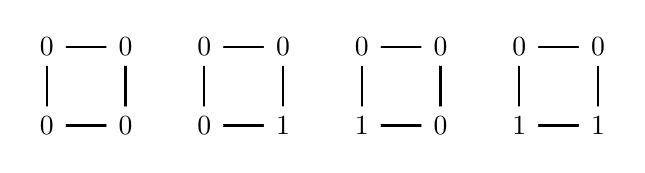
\begin{tikzpicture}
        % row1
        \cell{0}{0}{1}{1}
        \cell{2}{0}{3}{1}
        \cell{4}{0}{5}{1}
        \cell{6}{0}{7}{1}

        \( \lablvertex{0}{0}{$0$} \)
        \( \lablvertex{1}{0}{$0$} \)
        \( \lablvertex{2}{0}{$0$} \)
        \( \lablvertex{3}{0}{$1$} \)
        \( \lablvertex{4}{0}{$1$} \)
        \( \lablvertex{5}{0}{$0$} \)
        \( \lablvertex{6}{0}{$1$} \)
        \( \lablvertex{7}{0}{$1$} \)

        \( \lablvertex{0}{1}{$0$} \)
        \( \lablvertex{1}{1}{$0$} \)
        \( \lablvertex{2}{1}{$0$} \)
        \( \lablvertex{3}{1}{$0$} \)
        \( \lablvertex{4}{1}{$0$} \)
        \( \lablvertex{5}{1}{$0$} \)
        \( \lablvertex{6}{1}{$0$} \)
        \( \lablvertex{7}{1}{$0$} \)
        
    \end{tikzpicture}
\end{center}

For example, for the $m=2$ column with index $(0,1)$, this operation looks like the following.

\begin{center}
    \begin{tikzpicture}
        % row1
        \cell{-4.5}{2.5}{-3.5}{3.5}
        \cell{-4.5}{3.5}{-3.5}{4.5}

        % row 1
        \( \lablvertex{-4.5}{2.5}{$0$} \)
        \( \lablvertex{-4.5}{3.5}{$0$} \)
        \( \lablvertex{-4.5}{4.5}{$0$} \)
        
        \( \lablvertex{-3.5}{2.5}{$0$} \)
        \( \lablvertex{-3.5}{3.5}{$1$} \)
        \( \lablvertex{-3.5}{4.5}{$0$} \)

        % label
        \( \lablnode{-4}{1.5}{$A(2)_{0,1}$} \)

        % arrow
        \( \lablnode{-2}{3.5}{$\pmb{\to}$} \)

        % four columns
        \cell{0}{0}{1}{1}
        \cell{0}{1}{1}{2}
        \cell{0}{2}{1}{3}

        \cell{2}{0}{3}{1}
        \cell{2}{1}{3}{2}
        \cell{2}{2}{3}{3}

        \( \lablvertex{0}{0}{$0$} \)
        \( \lablvertex{0}{1}{$0$} \)
        \( \lablvertex{0}{2}{$1$} \)
        \( \lablvertex{0}{3}{$0$} \)
        
        \( \lablvertex{1}{0}{$0$} \)
        \( \lablvertex{1}{1}{$1$} \)
        \( \lablvertex{1}{2}{$0$} \)
        \( \lablvertex{1}{3}{$0$} \)
        
        \( \lablvertex{2}{0}{$0$} \)
        \( \lablvertex{2}{1}{$0$} \)
        \( \lablvertex{2}{2}{$1$} \)
        \( \lablvertex{2}{3}{$0$} \)
        
        \( \lablvertex{3}{0}{$0$} \)
        \( \lablvertex{3}{1}{$1$} \)
        \( \lablvertex{3}{2}{$1$} \)
        \( \lablvertex{3}{3}{$0$} \)
        
        \cell{0}{4}{1}{5}
        \cell{0}{5}{1}{6}
        \cell{0}{6}{1}{7}
        
        \cell{2}{4}{3}{5}
        \cell{2}{5}{3}{6}
        \cell{2}{6}{3}{7}

        \( \lablvertex{0}{4}{$0$} \)
        \( \lablvertex{0}{5}{$0$} \)
        \( \lablvertex{0}{6}{$0$} \)
        \( \lablvertex{0}{7}{$0$} \)
        
        \( \lablvertex{1}{4}{$0$} \)
        \( \lablvertex{1}{5}{$1$} \)
        \( \lablvertex{1}{6}{$0$} \)
        \( \lablvertex{1}{7}{$0$} \)
        
        \( \lablvertex{2}{4}{$0$} \)
        \( \lablvertex{2}{5}{$0$} \)
        \( \lablvertex{2}{6}{$0$} \)
        \( \lablvertex{2}{7}{$0$} \)
        
        \( \lablvertex{3}{4}{$0$} \)
        \( \lablvertex{3}{5}{$1$} \)
        \( \lablvertex{3}{6}{$1$} \)
        \( \lablvertex{3}{7}{$0$} \)

        \( \lablnode{5}{3.5}{$\pmb{\to}$} \)

        \( \lablnode{7.5}{3.5}{$\begin{bmatrix} A(3)_{0,2} & A(3)_{0,3} \\ A(3)_{1,2} & A(3)_{1,3} \end{bmatrix}$} \)

    \end{tikzpicture}
\end{center}

This operation results in $4$ new columns that are represented in $A(k+1)$. In our example, specifically we get the following. 

$$
\begin{bmatrix} 
    A(3)_{0,2} & A(3)_{0,3} \\ 
    A(3)_{1,2} & A(3)_{1,3} 
\end{bmatrix} = 
\begin{bmatrix} 
    1A(2)_{i,j} & 1A(2)_{i,j} \\ 
    0A(2)_{i,j} & 1A(2)_{i,j} 
\end{bmatrix},
$$

Critically, this transformation \textit{only} changes the identity of the top two tiles. This implies that the same value coefficients computed by comparing $A(2)$ and $A(3)$ can be used for any $m \times 1$ column, as long as both column indices $(i,j)$ are congruent $\text{mod } 2$. Furthermore, if one writes $A(k)$ as the block matrix

$$A(k) = \begin{bmatrix} A_{0,0} & A_{0,1} \\ A_{1,0} & A_{1,1} \end{bmatrix},$$

where $A_{\hat{i},\hat{j}} \in \mathbb{R}^{2^{k-2} \times 2^{k-2}}$, then all column's represented in $A_{\hat{i},\hat{j}}$ have indices $(i,j) \equiv (\hat{i},\hat{j}) \text{ mod } 2$. This allows us to write that in general, if $A(k) = \begin{bmatrix} A_{0,0} & A_{0,1} \\ A_{1,0} & A_{1,1} \end{bmatrix},$
then

\begin{equation}\label{eqn: coefficient matrix prod}
    \begin{bmatrix}
        V_{0,0}A_{0,0} & V_{0,1}A_{0,0} & V_{0,2}A_{0,1} & V_{0,3}A_{0,1} \\
        V_{1,0}A_{0,0} & V_{1,1}A_{0,0} & V_{1,2}A_{0,1} & V_{1,3}A_{0,1} \\
        V_{2,0}A_{1,0} & V_{2,1}A_{1,0} & V_{2,2}A_{1,1} & V_{2,3}A_{1,1} \\
        V_{3,0}A_{1,0} & V_{3,1}A_{1,0} & V_{3,2}A_{1,1} & V_{3,3}A_{1,1} \\
    \end{bmatrix}.
\end{equation}


where $V \in \mathbb{R}^{4 \times 4}$ can be found after directly computing $A(2)$ and $A(3)$, then solving the following equation.

$$
\begin{bmatrix}
    A(3)_{0,0} & A(3)_{0,1} & A(3)_{0,2} & A(3)_{0,3} \\
    A(3)_{1,0} & A(3)_{1,1} & A(3)_{1,2} & A(3)_{1,3} \\
    A(3)_{2,0} & A(3)_{2,1} & A(3)_{2,2} & A(3)_{2,3} \\
    A(3)_{3,0} & A(3)_{3,1} & A(3)_{3,2} & A(3)_{3,3} \\
\end{bmatrix} = 
\begin{bmatrix}
    V_{0,0}A(2)_{0,0} & V_{0,1}A(2)_{0,0} & V_{0,2}A(2)_{0,1} & V_{0,3}A(2)_{0,1} \\
    V_{1,0}A(2)_{0,0} & V_{1,1}A(2)_{0,0} & V_{1,2}A(2)_{0,1} & V_{1,3}A(2)_{0,1} \\
    V_{2,0}A(2)_{1,0} & V_{2,1}A(2)_{1,0} & V_{2,2}A(2)_{1,1} & V_{2,3}A(2)_{1,1} \\
    V_{3,0}A(2)_{1,0} & V_{3,1}A(2)_{1,0} & V_{3,2}A(2)_{1,1} & V_{3,3}A(2)_{1,1} \\
\end{bmatrix}
$$

This is solved by

$$V = 
\begin{bmatrix} 
    1 & 1 & 1 & 1 \\ 
    1 & 1 & 0 & 1 \\ 
    1 & 0 & 1 & 1 \\ 
    1 & 1 & 1 & 1 
\end{bmatrix}
$$


which completes the proof.

% \end{proof}

The method detailed in Theorem \ref{thm: main theorem} generalizes to other tile sets, which we tabularize in Section \ref{section: summary of results} without proof. Interestingly, the method not only generalizes to other tile sets, but can also be augmented to enumerate the more complicated ``messy" polygon mosaics.



As demonstrated in the proof of Theorem \ref{thm: messy mosaics}, the enumeration of both polygon mosaics and mosaics that do not contain a polygon share the same structure, and only differ by the identity of the matrices $A(2), V$. We summarize these matrices for various collections of tiles below.

\section{OLD STUFF}

\begin{proof}
We consider the same vertex labeling in the proof of Theorem \ref{thm: main theorem}, namely labeling a vertex by the number of polygons that contain it $\text{mod } 2$. Though avoided in the previous proof for clarity, it is important to think of each individual cell labeling as having its own weight, which corresponds with how many distinct tiles can map to the cell labeling.

\begin{center}
    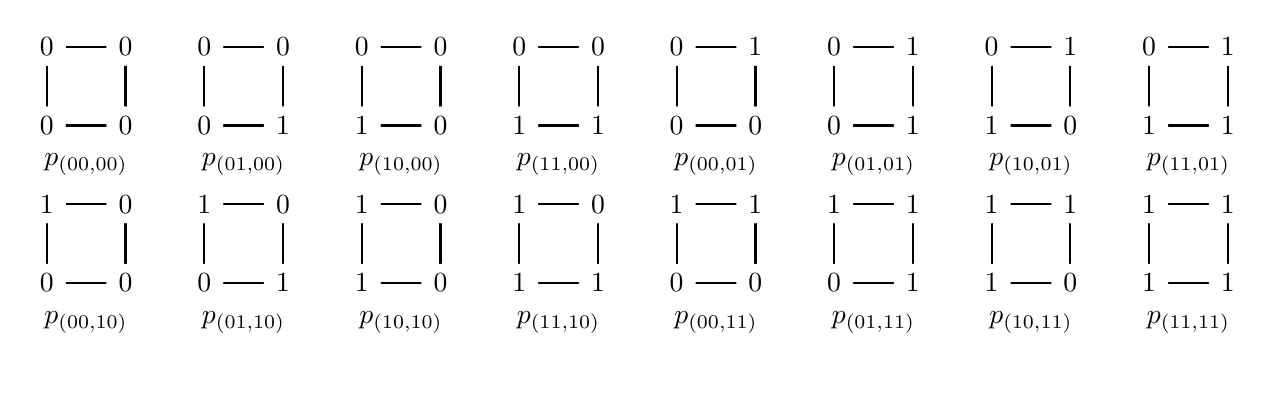
\begin{tikzpicture}
        % row1
        \cell{0}{0}{1}{1}
        \cell{2}{0}{3}{1}
        \cell{4}{0}{5}{1}
        \cell{6}{0}{7}{1}
        \cell{8}{0}{9}{1}
        \cell{10}{0}{11}{1}
        \cell{12}{0}{13}{1}
        \cell{14}{0}{15}{1}
        % row2
        \cell{0}{2}{1}{3}
        \cell{2}{2}{3}{3}
        \cell{4}{2}{5}{3}
        \cell{6}{2}{7}{3}
        \cell{8}{2}{9}{3}
        \cell{10}{2}{11}{3}
        \cell{12}{2}{13}{3}
        \cell{14}{2}{15}{3}

        % label for row1
        \( \lablvertex{0}{0}{$0$} \)
        \( \lablvertex{1}{0}{$0$} \)
        \( \lablvertex{2}{0}{$0$} \)
        \( \lablvertex{3}{0}{$1$} \)
        \( \lablvertex{4}{0}{$1$} \)
        \( \lablvertex{5}{0}{$0$} \)
        \( \lablvertex{6}{0}{$1$} \)
        \( \lablvertex{7}{0}{$1$} \)
        \( \lablvertex{8}{0}{$0$} \)
        \( \lablvertex{9}{0}{$0$} \)
        \( \lablvertex{10}{0}{$0$} \)
        \( \lablvertex{11}{0}{$1$} \)
        \( \lablvertex{12}{0}{$1$} \)
        \( \lablvertex{13}{0}{$0$} \)
        \( \lablvertex{14}{0}{$1$} \)
        \( \lablvertex{15}{0}{$1$} \)
        
        % label for row1
        \( \lablvertex{0}{1}{$1$} \)
        \( \lablvertex{1}{1}{$0$} \)
        \( \lablvertex{2}{1}{$1$} \)
        \( \lablvertex{3}{1}{$0$} \)
        \( \lablvertex{4}{1}{$1$} \)
        \( \lablvertex{5}{1}{$0$} \)
        \( \lablvertex{6}{1}{$1$} \)
        \( \lablvertex{7}{1}{$0$} \)
        \( \lablvertex{8}{1}{$1$} \)
        \( \lablvertex{9}{1}{$1$} \)
        \( \lablvertex{10}{1}{$1$} \)
        \( \lablvertex{11}{1}{$1$} \)
        \( \lablvertex{12}{1}{$1$} \)
        \( \lablvertex{13}{1}{$1$} \)
        \( \lablvertex{14}{1}{$1$} \)
        \( \lablvertex{15}{1}{$1$} \)

        \( \lablvertex{0}{2}{$0$} \)
        \( \lablvertex{1}{2}{$0$} \)
        \( \lablvertex{2}{2}{$0$} \)
        \( \lablvertex{3}{2}{$1$} \)
        \( \lablvertex{4}{2}{$1$} \)
        \( \lablvertex{5}{2}{$0$} \)
        \( \lablvertex{6}{2}{$1$} \)
        \( \lablvertex{7}{2}{$1$} \)
        \( \lablvertex{8}{2}{$0$} \)
        \( \lablvertex{9}{2}{$0$} \)
        \( \lablvertex{10}{2}{$0$} \)
        \( \lablvertex{11}{2}{$1$} \)
        \( \lablvertex{12}{2}{$1$} \)
        \( \lablvertex{13}{2}{$0$} \)
        \( \lablvertex{14}{2}{$1$} \)
        \( \lablvertex{15}{2}{$1$} \)

        \( \lablvertex{0}{3}{$0$} \)
        \( \lablvertex{1}{3}{$0$} \)
        \( \lablvertex{2}{3}{$0$} \)
        \( \lablvertex{3}{3}{$0$} \)
        \( \lablvertex{4}{3}{$0$} \)
        \( \lablvertex{5}{3}{$0$} \)
        \( \lablvertex{6}{3}{$0$} \)
        \( \lablvertex{7}{3}{$0$} \)
        \( \lablvertex{8}{3}{$0$} \)
        \( \lablvertex{9}{3}{$1$} \)
        \( \lablvertex{10}{3}{$0$} \)
        \( \lablvertex{11}{3}{$1$} \)
        \( \lablvertex{12}{3}{$0$} \)
        \( \lablvertex{13}{3}{$1$} \)
        \( \lablvertex{14}{3}{$0$} \)
        \( \lablvertex{15}{3}{$1$} \)

        % numbers row 1
        \( \lablnode{0.5}{-0.5}{$p_{(00,10)}$} \)
        \( \lablnode{2.5}{-0.5}{$p_{(01,10)}$} \)
        \( \lablnode{4.5}{-0.5}{$p_{(10,10)}$} \)
        \( \lablnode{6.5}{-0.5}{$p_{(11,10)}$} \)
        \( \lablnode{8.5}{-0.5}{$p_{(00,11)}$} \)
        \( \lablnode{10.5}{-0.5}{$p_{(01,11)}$} \)
        \( \lablnode{12.5}{-0.5}{$p_{(10,11)}$} \)
        \( \lablnode{14.5}{-0.5}{$p_{(11,11)}$} \)
        % numbers row 2
        \( \lablnode{0.5}{1.5}{$p_{(00,00)}$} \)
        \( \lablnode{2.5}{1.5}{$p_{(01,00)}$} \)
        \( \lablnode{4.5}{1.5}{$p_{(10,00)}$} \)
        \( \lablnode{6.5}{1.5}{$p_{(11,00)}$} \)
        \( \lablnode{8.5}{1.5}{$p_{(00,01)}$} \)
        \( \lablnode{10.5}{1.5}{$p_{(01,01)}$} \)
        \( \lablnode{12.5}{1.5}{$p_{(10,01)}$} \)
        \( \lablnode{14.5}{1.5}{$p_{(11,01)}$} \)
    \end{tikzpicture}
\end{center}

The proof of Theorem \ref{thm: main theorem} can be seen as assigning $p_{(10,01)} = p_{(01,10)} = 0$, and all other weights to $1$. The usefulness of this view can be seen when considering the operation for creating the recursive definition for $A(k)$ in the previous proof. Previously, we defined the coefficient matrix $V$ by computing $A(2)$ and $A(3)$ directly and comparing. Now with a weight assigned to individual cell labelings, we can define the values of $A(2)$ and $V$ directly in terms of these weights.

$$
A(2) = 
\begin{bmatrix}
    p_{(00,00)}p_{(00,00)} & p_{(01,00)} p_{(00,01)} \\
    p_{(10,00)} p_{(00,10)} & p_{(11,00)} p_{(00,11)}
\end{bmatrix},
V = 
\begin{bmatrix}
    \frac{p_{(00,00)} p_{(00,00)}}{p_{(00,00)}} & \frac{p_{(01,00)} p_{(00,01)}}{p_{(00,00)}} & \frac{p_{(00,00)} p_{(01,00)}}{p_{(01,00)}} & \frac{p_{(01,00)} p_{(01,01)}}{p_{(01,00)}} \\
    \frac{p_{(10,00)} p_{(00,10)}}{p_{(00,00)}} & \frac{p_{(11,00)} p_{(00,11)}}{p_{(00,00)}} & \frac{p_{(10,00)} p_{(01,10)}}{p_{(01,00)}} & \frac{p_{(11,00)} p_{(01,11)}}{p_{(01,00)}} \\
    \frac{p_{(00,00)} p_{(10,00)}}{p_{(10,00)}} & \frac{p_{(01,00)} p_{(10,01)}}{p_{(10,00)}} & \frac{p_{(00,00)} p_{(11,00)}}{p_{(11,00)}} & \frac{p_{(01,00)} p_{(11,01)}}{p_{(11,00)}} \\
    \frac{p_{(10,00)} p_{(10,10)}}{p_{(10,00)}} & \frac{p_{(11,00)} p_{(10,11)}}{p_{(10,00)}} & \frac{p_{(10,00)} p_{(11,10)}}{p_{(11,00)}} & \frac{p_{(11,00)} p_{(11,11)}}{p_{(11,00)}}
\end{bmatrix}
= 
\begin{bmatrix}
    p_{(00,00)} & \frac{p_{(01,00)} p_{(00,01)}}{p_{(00,00)}} & p_{(00,00)} & p_{(01,01)} \\
    \frac{p_{(10,00)} p_{(00,10)}}{p_{(00,00)}} & \frac{p_{(11,00)} p_{(00,11)}}{p_{(00,00)}} & \frac{p_{(10,00)} p_{(01,10)}}{p_{(01,00)}} & \frac{p_{(11,00)} p_{(01,11)}}{p_{(01,00)}} \\
    p_{(00,00)} & \frac{p_{(01,00)} p_{(10,01)}}{p_{(10,00)}} & p_{(00,00)} & \frac{p_{(01,00)} p_{(11,01)}}{p_{(11,00)}} \\
    p_{(10,10)} & \frac{p_{(11,00)} p_{(10,11)}}{p_{(10,00)}} & \frac{p_{(10,00)} p_{(11,10)}}{p_{(11,00)}} & p_{(11,11)}
\end{bmatrix}.
$$

With this identity, we can enumerate $t_{m,n}$ once we have proper assignments for the $16$ weights. As in the previous proof, we have $p_{(10,01)}=p_{(01,10)}=0$, as again these are impossible vertex labelings for our tile set. 

Next consider the cell labelings for $p_{(00,00)}$ and $p_{(11,11)}$. When enumerating polygon mosaics (and their messy variant), these cell labelings do not contribute to the cells of a polygon. For polygon mosaics, only the $T_1$ tile are permitted to not contribute to the shape of a polygon. However, in messy polygon mosaics, all $7$ tiles are permitted to not contribute to the shape of the polygon, so $p_{(00,00)} = p_{(11,11)}=7$.

However, this means we now lose the uniqueness of the map from vertex labeling to messy polygon mosaics. For instance, the sub-grid vertex labelings below are now ambiguous as to whether or not they represent a polygon.

\begin{center}
    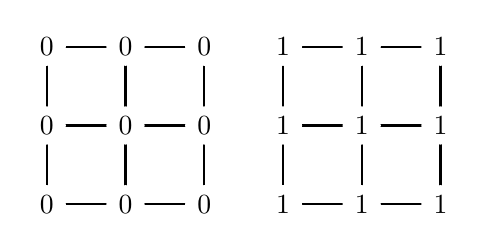
\begin{tikzpicture}
        % row1
        \cell{0}{0}{1}{1}
        \cell{0}{1}{1}{2}
        \cell{1}{0}{2}{1}
        \cell{1}{1}{2}{2}

        \( \lablvertex{0}{0}{$0$} \)
        \( \lablvertex{1}{0}{$0$} \)
        \( \lablvertex{2}{0}{$0$} \)

        \( \lablvertex{0}{1}{$0$} \)
        \( \lablvertex{1}{1}{$0$} \)
        \( \lablvertex{2}{1}{$0$} \)
        
        \( \lablvertex{0}{2}{$0$} \)
        \( \lablvertex{1}{2}{$0$} \)
        \( \lablvertex{2}{2}{$0$} \)
        
        % row1
        \cell{3}{0}{4}{1}
        \cell{3}{1}{4}{2}
        \cell{4}{0}{5}{1}
        \cell{4}{1}{5}{2}

        \( \lablvertex{3}{0}{$1$} \)
        \( \lablvertex{4}{0}{$1$} \)
        \( \lablvertex{5}{0}{$1$} \)

        \( \lablvertex{3}{1}{$1$} \)
        \( \lablvertex{4}{1}{$1$} \)
        \( \lablvertex{5}{1}{$1$} \)

        \( \lablvertex{3}{2}{$1$} \)
        \( \lablvertex{4}{2}{$1$} \)
        \( \lablvertex{5}{2}{$1$} \)

    \end{tikzpicture}
\end{center}

This ambiguity is explored in the following example.

\begin{exmp}\label{exmp: iep}

Consider the four vertex labelings below, along with the messy polygon mosaic on the right. Write the product of the weights of all cell labelings below each, assuming all weights not defined above are $1$.

\begin{center}
    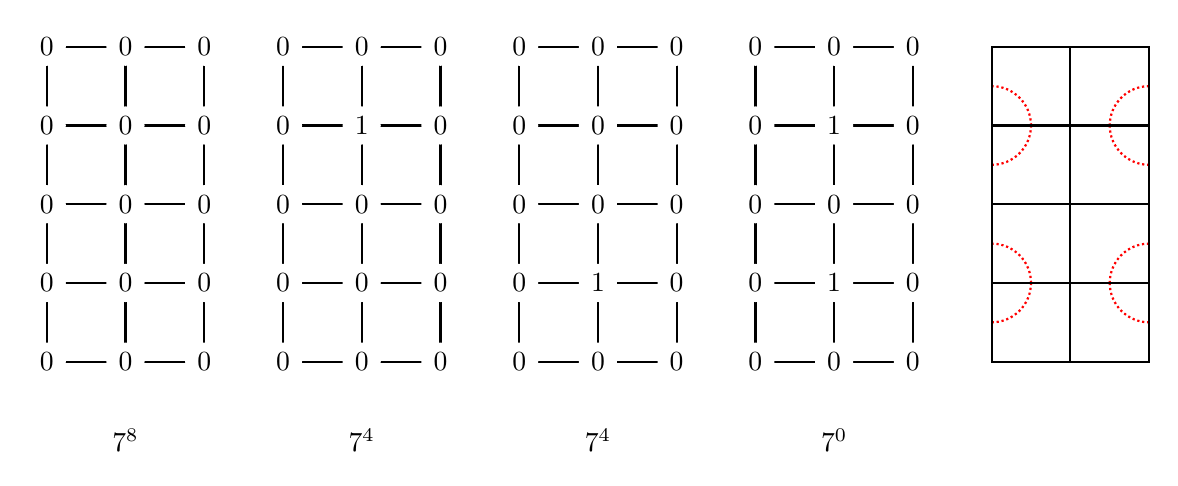
\begin{tikzpicture}
        % row1
        \cell{-6}{0}{-5}{1}
        \cell{-6}{1}{-5}{2}
        \cell{-6}{2}{-5}{3}
        \cell{-6}{3}{-5}{4}
        \cell{-5}{0}{-4}{1}
        \cell{-5}{1}{-4}{2}
        \cell{-5}{2}{-4}{3}
        \cell{-5}{3}{-4}{4}

        \( \lablnode{-5}{-1}{$7^8$} \)

        \( \lablvertex{-6}{0}{$0$} \)
        \( \lablvertex{-5}{0}{$0$} \)
        \( \lablvertex{-4}{0}{$0$} \)

        \( \lablvertex{-6}{1}{$0$} \)
        \( \lablvertex{-5}{1}{$0$} \)
        \( \lablvertex{-4}{1}{$0$} \)

        \( \lablvertex{-6}{2}{$0$} \)
        \( \lablvertex{-5}{2}{$0$} \)
        \( \lablvertex{-4}{2}{$0$} \)

        \( \lablvertex{-6}{3}{$0$} \)
        \( \lablvertex{-5}{3}{$0$} \)
        \( \lablvertex{-4}{3}{$0$} \)

        \( \lablvertex{-6}{4}{$0$} \)
        \( \lablvertex{-5}{4}{$0$} \)
        \( \lablvertex{-4}{4}{$0$} \)
        % row1
        \cell{-3}{0}{-2}{1}
        \cell{-3}{1}{-2}{2}
        \cell{-3}{2}{-2}{3}
        \cell{-3}{3}{-2}{4}
        \cell{-2}{0}{-1}{1}
        \cell{-2}{1}{-1}{2}
        \cell{-2}{2}{-1}{3}
        \cell{-2}{3}{-1}{4}

        \( \lablnode{-2}{-1}{$7^4$} \)

        \( \lablvertex{-3}{0}{$0$} \)
        \( \lablvertex{-2}{0}{$0$} \)
        \( \lablvertex{-1}{0}{$0$} \)

        \( \lablvertex{-3}{1}{$0$} \)
        \( \lablvertex{-2}{1}{$0$} \)
        \( \lablvertex{-1}{1}{$0$} \)

        \( \lablvertex{-3}{2}{$0$} \)
        \( \lablvertex{-2}{2}{$0$} \)
        \( \lablvertex{-1}{2}{$0$} \)

        \( \lablvertex{-3}{3}{$0$} \)
        \( \lablvertex{-2}{3}{$1$} \)
        \( \lablvertex{-1}{3}{$0$} \)

        \( \lablvertex{-3}{4}{$0$} \)
        \( \lablvertex{-2}{4}{$0$} \)
        \( \lablvertex{-1}{4}{$0$} \)

        % row1
        \cell{0}{0}{1}{1}
        \cell{0}{1}{1}{2}
        \cell{0}{2}{1}{3}
        \cell{0}{3}{1}{4}
        \cell{1}{0}{2}{1}
        \cell{1}{1}{2}{2}
        \cell{1}{2}{2}{3}
        \cell{1}{3}{2}{4}

        \( \lablnode{1}{-1}{$7^4$} \)
        
        \( \lablvertex{0}{0}{$0$} \)
        \( \lablvertex{1}{0}{$0$} \)
        \( \lablvertex{2}{0}{$0$} \)

        \( \lablvertex{0}{1}{$0$} \)
        \( \lablvertex{1}{1}{$1$} \)
        \( \lablvertex{2}{1}{$0$} \)

        \( \lablvertex{0}{2}{$0$} \)
        \( \lablvertex{1}{2}{$0$} \)
        \( \lablvertex{2}{2}{$0$} \)

        \( \lablvertex{0}{3}{$0$} \)
        \( \lablvertex{1}{3}{$0$} \)
        \( \lablvertex{2}{3}{$0$} \)

        \( \lablvertex{0}{4}{$0$} \)
        \( \lablvertex{1}{4}{$0$} \)
        \( \lablvertex{2}{4}{$0$} \)

        % row1
        \cell{3}{0}{4}{1}
        \cell{3}{1}{4}{2}
        \cell{3}{2}{4}{3}
        \cell{3}{3}{4}{4}
        \cell{4}{0}{5}{1}
        \cell{4}{1}{5}{2}
        \cell{4}{2}{5}{3}
        \cell{4}{3}{5}{4}

        \( \lablnode{4}{-1}{$7^0$} \)

        \( \lablvertex{3}{0}{$0$} \)
        \( \lablvertex{4}{0}{$0$} \)
        \( \lablvertex{5}{0}{$0$} \)

        \( \lablvertex{3}{1}{$0$} \)
        \( \lablvertex{4}{1}{$1$} \)
        \( \lablvertex{5}{1}{$0$} \)

        \( \lablvertex{3}{2}{$0$} \)
        \( \lablvertex{4}{2}{$0$} \)
        \( \lablvertex{5}{2}{$0$} \)

        \( \lablvertex{3}{3}{$0$} \)
        \( \lablvertex{4}{3}{$1$} \)
        \( \lablvertex{5}{3}{$0$} \)

        \( \lablvertex{3}{4}{$0$} \)
        \( \lablvertex{4}{4}{$0$} \)
        \( \lablvertex{5}{4}{$0$} \)

        \cellD{6}{0}{7}{1}
        \cellC{7}{0}{8}{1}

        \cellA{6}{1}{7}{2}
        \cellB{7}{1}{8}{2}

        \cellD{6}{2}{7}{3}
        \cellC{7}{2}{8}{3}    

        \cellA{6}{3}{7}{4}
        \cellB{7}{3}{8}{4}    

    \end{tikzpicture}
\end{center}

Notice that each vertex labeling could include the right-most messy polygon mosaic. In fact, the left-most vertex labeling contains all possible mosaics! If we were to add these weight products together, we would count the right messy polygon mosaic $4$ times.

\end{exmp}

The double counting demonstrated in Example \ref{exmp: iep} motivates the following idea. If vertex labelings with an odd number of polygons are negative, then the addition of these weight products would incorporate the \textit{inclusion-exclusion principle}, mitigating the double counting. In Example \ref{exmp: iep}, the sum $7^8 - 7^4 - 7^4 + 7^0$ would then represent the number of mosaics that \textit{do not} contain the following three classes of messy polygon mosaics, where cells that can be any tile are marked with a dot.

\begin{center}
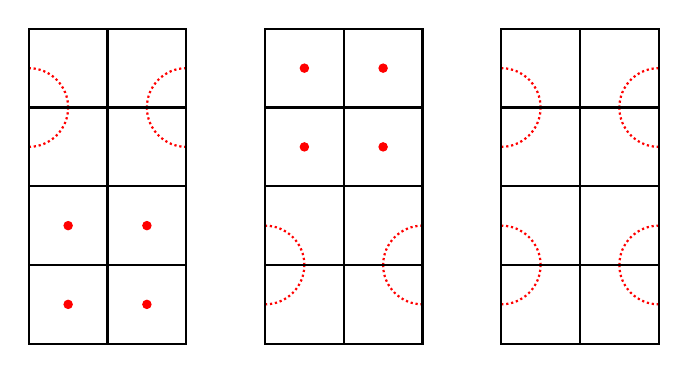
\begin{tikzpicture}
    %
    \cellopen{0}{0}{1}{1}
    \cellopen{1}{0}{2}{1}

    \cellopen{0}{1}{1}{2}
    \cellopen{1}{1}{2}{2}

    \cellD{0}{2}{1}{3}
    \cellC{1}{2}{2}{3}    

    \cellA{0}{3}{1}{4}
    \cellB{1}{3}{2}{4}
    %
    \cellD{3}{0}{4}{1}
    \cellC{4}{0}{5}{1}

    \cellA{3}{1}{4}{2}
    \cellB{4}{1}{5}{2}

    \cellopen{3}{2}{4}{3}
    \cellopen{4}{2}{5}{3}    

    \cellopen{3}{3}{4}{4}
    \cellopen{4}{3}{5}{4}
    %
    \cellD{6}{0}{7}{1}
    \cellC{7}{0}{8}{1}

    \cellA{6}{1}{7}{2}
    \cellB{7}{1}{8}{2}

    \cellD{6}{2}{7}{3}
    \cellC{7}{2}{8}{3}    

    \cellA{6}{3}{7}{4}
    \cellB{7}{3}{8}{4}
\end{tikzpicture}
\end{center}

Therefore, the sum over the products for all vertex labelings, where the product is negative if the vertex labeling represents an odd number of polygons in the mosaic, would be the number of mosaics that \textit{do not} include messy polygon mosaics.

We can accomplish this by finding a weight assignment such that the product over the cell labeling weights of \textit{any} single polygon equals $-1$. It is not obvious that such an assignment can even be found! 

Luckily such assignments exist. The proof of this fact can be found in the Appendix, and choosing an assignment gives us the following weight assignments.

\begin{center}
    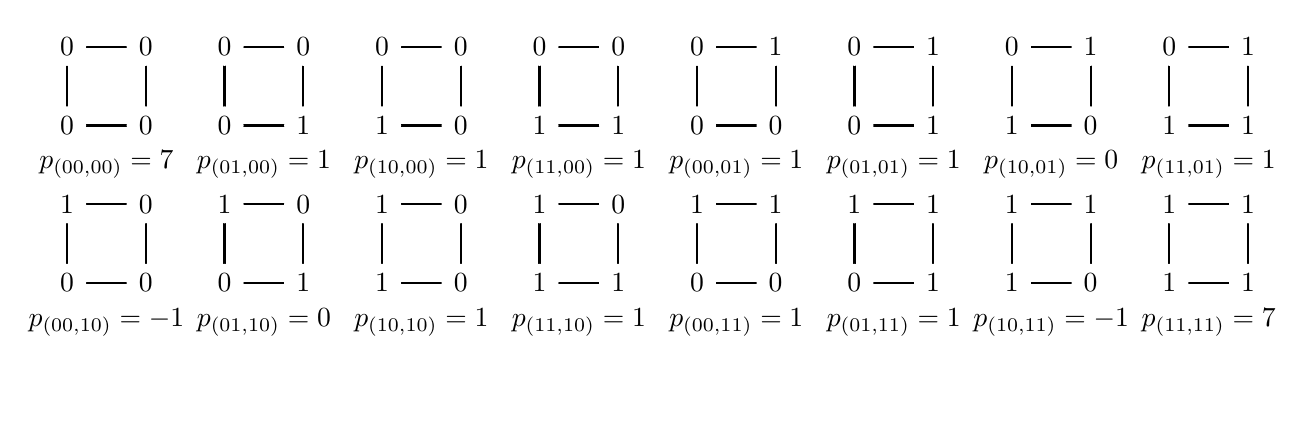
\begin{tikzpicture}
        % row1
        \cell{0}{0}{1}{1}
        \cell{2}{0}{3}{1}
        \cell{4}{0}{5}{1}
        \cell{6}{0}{7}{1}
        \cell{8}{0}{9}{1}
        \cell{10}{0}{11}{1}
        \cell{12}{0}{13}{1}
        \cell{14}{0}{15}{1}
        % row2
        \cell{0}{2}{1}{3}
        \cell{2}{2}{3}{3}
        \cell{4}{2}{5}{3}
        \cell{6}{2}{7}{3}
        \cell{8}{2}{9}{3}
        \cell{10}{2}{11}{3}
        \cell{12}{2}{13}{3}
        \cell{14}{2}{15}{3}

        % label for row1
        \( \lablvertex{0}{0}{$0$} \)
        \( \lablvertex{1}{0}{$0$} \)
        \( \lablvertex{2}{0}{$0$} \)
        \( \lablvertex{3}{0}{$1$} \)
        \( \lablvertex{4}{0}{$1$} \)
        \( \lablvertex{5}{0}{$0$} \)
        \( \lablvertex{6}{0}{$1$} \)
        \( \lablvertex{7}{0}{$1$} \)
        \( \lablvertex{8}{0}{$0$} \)
        \( \lablvertex{9}{0}{$0$} \)
        \( \lablvertex{10}{0}{$0$} \)
        \( \lablvertex{11}{0}{$1$} \)
        \( \lablvertex{12}{0}{$1$} \)
        \( \lablvertex{13}{0}{$0$} \)
        \( \lablvertex{14}{0}{$1$} \)
        \( \lablvertex{15}{0}{$1$} \)
        
        % label for row1
        \( \lablvertex{0}{1}{$1$} \)
        \( \lablvertex{1}{1}{$0$} \)
        \( \lablvertex{2}{1}{$1$} \)
        \( \lablvertex{3}{1}{$0$} \)
        \( \lablvertex{4}{1}{$1$} \)
        \( \lablvertex{5}{1}{$0$} \)
        \( \lablvertex{6}{1}{$1$} \)
        \( \lablvertex{7}{1}{$0$} \)
        \( \lablvertex{8}{1}{$1$} \)
        \( \lablvertex{9}{1}{$1$} \)
        \( \lablvertex{10}{1}{$1$} \)
        \( \lablvertex{11}{1}{$1$} \)
        \( \lablvertex{12}{1}{$1$} \)
        \( \lablvertex{13}{1}{$1$} \)
        \( \lablvertex{14}{1}{$1$} \)
        \( \lablvertex{15}{1}{$1$} \)

        \( \lablvertex{0}{2}{$0$} \)
        \( \lablvertex{1}{2}{$0$} \)
        \( \lablvertex{2}{2}{$0$} \)
        \( \lablvertex{3}{2}{$1$} \)
        \( \lablvertex{4}{2}{$1$} \)
        \( \lablvertex{5}{2}{$0$} \)
        \( \lablvertex{6}{2}{$1$} \)
        \( \lablvertex{7}{2}{$1$} \)
        \( \lablvertex{8}{2}{$0$} \)
        \( \lablvertex{9}{2}{$0$} \)
        \( \lablvertex{10}{2}{$0$} \)
        \( \lablvertex{11}{2}{$1$} \)
        \( \lablvertex{12}{2}{$1$} \)
        \( \lablvertex{13}{2}{$0$} \)
        \( \lablvertex{14}{2}{$1$} \)
        \( \lablvertex{15}{2}{$1$} \)

        \( \lablvertex{0}{3}{$0$} \)
        \( \lablvertex{1}{3}{$0$} \)
        \( \lablvertex{2}{3}{$0$} \)
        \( \lablvertex{3}{3}{$0$} \)
        \( \lablvertex{4}{3}{$0$} \)
        \( \lablvertex{5}{3}{$0$} \)
        \( \lablvertex{6}{3}{$0$} \)
        \( \lablvertex{7}{3}{$0$} \)
        \( \lablvertex{8}{3}{$0$} \)
        \( \lablvertex{9}{3}{$1$} \)
        \( \lablvertex{10}{3}{$0$} \)
        \( \lablvertex{11}{3}{$1$} \)
        \( \lablvertex{12}{3}{$0$} \)
        \( \lablvertex{13}{3}{$1$} \)
        \( \lablvertex{14}{3}{$0$} \)
        \( \lablvertex{15}{3}{$1$} \)

        % numbers row 1
        \( \lablnode{0.5}{-0.5}{$p_{(00,10)}=-1$} \)
        \( \lablnode{2.5}{-0.5}{$p_{(01,10)}=0$} \)
        \( \lablnode{4.5}{-0.5}{$p_{(10,10)}=1$} \)
        \( \lablnode{6.5}{-0.5}{$p_{(11,10)}=1$} \)
        \( \lablnode{8.5}{-0.5}{$p_{(00,11)}=1$} \)
        \( \lablnode{10.5}{-0.5}{$p_{(01,11)}=1$} \)
        \( \lablnode{12.5}{-0.5}{$p_{(10,11)}=-1$} \)
        \( \lablnode{14.5}{-0.5}{$p_{(11,11)}=7$} \)
        % numbers row 2
        \( \lablnode{0.5}{1.5}{$p_{(00,00)}=7$} \)
        \( \lablnode{2.5}{1.5}{$p_{(01,00)}=1$} \)
        \( \lablnode{4.5}{1.5}{$p_{(10,00)}=1$} \)
        \( \lablnode{6.5}{1.5}{$p_{(11,00)}=1$} \)
        \( \lablnode{8.5}{1.5}{$p_{(00,01)}=1$} \)
        \( \lablnode{10.5}{1.5}{$p_{(01,01)}=1$} \)
        \( \lablnode{12.5}{1.5}{$p_{(10,01)}=0$} \)
        \( \lablnode{14.5}{1.5}{$p_{(11,01)}=1$} \)
    \end{tikzpicture}
\end{center}

This immediately gives us a way to construct an analagous definition for $A(k+1)$ given $A(k)$. Once we write $A(k) = \begin{bmatrix} A_{0,0} & A_{0,1} \\ A_{1,0} & A_{1,1} \end{bmatrix}$, we have

$$
A(2) = 
\begin{bmatrix}
    7^2 & 1 \\
    -1 & 1
\end{bmatrix},
V = 
\begin{bmatrix}
    7 & \frac{1}{7} & 7 & 1 \\
    -\frac{1}{7} & 1 & 0 & 1 \\
    7 & 0 & 7  & 1 \\
    1 & -1 & 1 & 7 \\
\end{bmatrix}
$$

Subsituting $V$ into Equation \ref{eqn: coefficient matrix prod} gives the result.

\end{proof}


Solving all Type 1 and Type 2 constraints gives the following solution set.

\begin{center}
\begin{tabular}{|c|c|c|c|c|c|c|c|c|c|c|c|c|c|c|c|} 
\hline
$w_{1}$ & $w_{2}$ & $w_{3}$ & $w_{4}$ & $w_{5}$ & $w_{6}$ & $w_{7}$ & $w_{8}$ & $w_{9}$ & $w_{10}$ & $w_{11}$ & $w_{12}$ & $w_{13}$ & $w_{14}$ & $w_{15}$ & $w_{16}$ \\
\hline
7 & -1 & -1 & -1 & -1 & -1 & 0 & -1 & 1 & 0 & -1 & -1 & -1 & -1 & 1 & 7 \\
7 & -1 & -1 & -1 & -1 & 1 & 0 & 1 & 1 & 0 & 1 & 1 & -1 & 1 & -1 & 7 \\
7 & -1 & -1 & -1 & 1 & -1 & 0 & -1 & -1 & 0 & -1 & -1 & -1 & 1 & -1 & 7 \\
7 & -1 & -1 & -1 & 1 & 1 & 0 & 1 & -1 & 0 & 1 & 1 & -1 & -1 & 1 & 7 \\
7 & -1 & -1 & 1 & -1 & -1 & 0 & 1 & 1 & 0 & -1 & 1 & 1 & 1 & -1 & 7 \\
7 & -1 & -1 & 1 & -1 & 1 & 0 & -1 & 1 & 0 & 1 & -1 & 1 & -1 & 1 & 7 \\
7 & -1 & -1 & 1 & 1 & -1 & 0 & 1 & -1 & 0 & -1 & 1 & 1 & -1 & 1 & 7 \\
7 & -1 & -1 & 1 & 1 & 1 & 0 & -1 & -1 & 0 & 1 & -1 & 1 & 1 & -1 & 7 \\
7 & -1 & 1 & -1 & -1 & -1 & 0 & -1 & -1 & 0 & -1 & 1 & -1 & -1 & -1 & 7 \\
7 & -1 & 1 & -1 & -1 & 1 & 0 & 1 & -1 & 0 & 1 & -1 & -1 & 1 & 1 & 7 \\
7 & -1 & 1 & -1 & 1 & -1 & 0 & -1 & 1 & 0 & -1 & 1 & -1 & 1 & 1 & 7 \\
7 & -1 & 1 & -1 & 1 & 1 & 0 & 1 & 1 & 0 & 1 & -1 & -1 & -1 & -1 & 7 \\
7 & -1 & 1 & 1 & -1 & -1 & 0 & 1 & -1 & 0 & -1 & -1 & 1 & 1 & 1 & 7 \\
7 & -1 & 1 & 1 & -1 & 1 & 0 & -1 & -1 & 0 & 1 & 1 & 1 & -1 & -1 & 7 \\
7 & -1 & 1 & 1 & 1 & -1 & 0 & 1 & 1 & 0 & -1 & -1 & 1 & -1 & -1 & 7 \\
7 & -1 & 1 & 1 & 1 & 1 & 0 & -1 & 1 & 0 & 1 & 1 & 1 & 1 & 1 & 7 \\
7 & 1 & -1 & -1 & -1 & -1 & 0 & 1 & -1 & 0 & -1 & -1 & -1 & -1 & -1 & 7 \\
7 & 1 & -1 & -1 & -1 & 1 & 0 & -1 & -1 & 0 & 1 & 1 & -1 & 1 & 1 & 7 \\
7 & 1 & -1 & -1 & 1 & -1 & 0 & 1 & 1 & 0 & -1 & -1 & -1 & 1 & 1 & 7 \\
7 & 1 & -1 & -1 & 1 & 1 & 0 & -1 & 1 & 0 & 1 & 1 & -1 & -1 & -1 & 7 \\
7 & 1 & -1 & 1 & -1 & -1 & 0 & -1 & -1 & 0 & -1 & 1 & 1 & 1 & 1 & 7 \\
7 & 1 & -1 & 1 & -1 & 1 & 0 & 1 & -1 & 0 & 1 & -1 & 1 & -1 & -1 & 7 \\
7 & 1 & -1 & 1 & 1 & -1 & 0 & -1 & 1 & 0 & -1 & 1 & 1 & -1 & -1 & 7 \\
7 & 1 & -1 & 1 & 1 & 1 & 0 & 1 & 1 & 0 & 1 & -1 & 1 & 1 & 1 & 7 \\
7 & 1 & 1 & -1 & -1 & -1 & 0 & 1 & 1 & 0 & -1 & 1 & -1 & -1 & 1 & 7 \\
7 & 1 & 1 & -1 & -1 & 1 & 0 & -1 & 1 & 0 & 1 & -1 & -1 & 1 & -1 & 7 \\
7 & 1 & 1 & -1 & 1 & -1 & 0 & 1 & -1 & 0 & -1 & 1 & -1 & 1 & -1 & 7 \\
7 & 1 & 1 & -1 & 1 & 1 & 0 & -1 & -1 & 0 & 1 & -1 & -1 & -1 & 1 & 7 \\
7 & 1 & 1 & 1 & -1 & -1 & 0 & -1 & 1 & 0 & -1 & -1 & 1 & 1 & -1 & 7 \\
7 & 1 & 1 & 1 & -1 & 1 & 0 & 1 & 1 & 0 & 1 & 1 & 1 & -1 & 1 & 7 \\
7 & 1 & 1 & 1 & 1 & -1 & 0 & -1 & -1 & 0 & -1 & -1 & 1 & -1 & 1 & 7 \\
7 & 1 & 1 & 1 & 1 & 1 & 0 & 1 & -1 & 0 & 1 & 1 & 1 & 1 & -1 & 7 \\
\hline
\end{tabular}
\end{center}

Any of these assignments are sufficient for calculating $t_{m,n}$. 



\begin{center}
    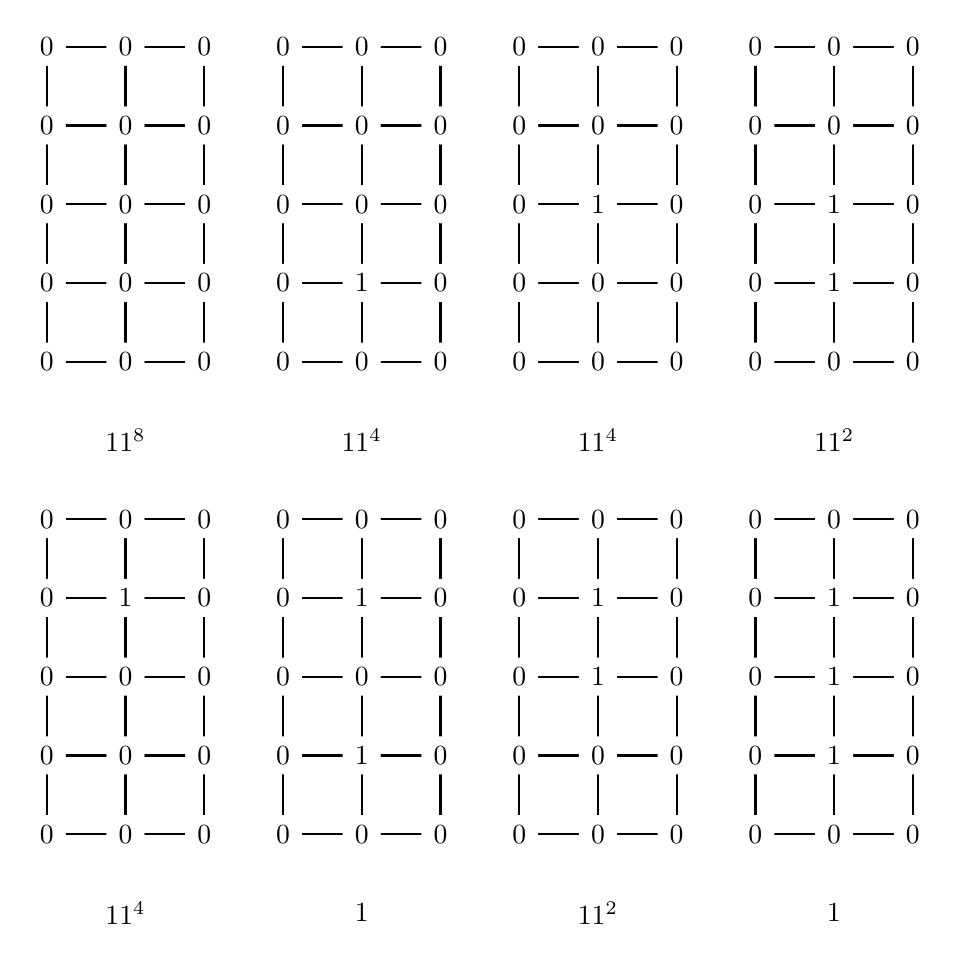
\begin{tikzpicture}
        % row1
        \cell{-6}{0}{-5}{1}
        \cell{-6}{1}{-5}{2}
        \cell{-6}{2}{-5}{3}
        \cell{-6}{3}{-5}{4}
        \cell{-5}{0}{-4}{1}
        \cell{-5}{1}{-4}{2}
        \cell{-5}{2}{-4}{3}
        \cell{-5}{3}{-4}{4}

        \( \lablnode{-5}{-1}{$11^4$} \)

        \( \lablvertex{-6}{0}{$0$} \)
        \( \lablvertex{-5}{0}{$0$} \)
        \( \lablvertex{-4}{0}{$0$} \)

        \( \lablvertex{-6}{1}{$0$} \)
        \( \lablvertex{-5}{1}{$0$} \)
        \( \lablvertex{-4}{1}{$0$} \)

        \( \lablvertex{-6}{2}{$0$} \)
        \( \lablvertex{-5}{2}{$0$} \)
        \( \lablvertex{-4}{2}{$0$} \)

        \( \lablvertex{-6}{3}{$0$} \)
        \( \lablvertex{-5}{3}{$1$} \)
        \( \lablvertex{-4}{3}{$0$} \)

        \( \lablvertex{-6}{4}{$0$} \)
        \( \lablvertex{-5}{4}{$0$} \)
        \( \lablvertex{-4}{4}{$0$} \)
        % row1
        \cell{-3}{0}{-2}{1}
        \cell{-3}{1}{-2}{2}
        \cell{-3}{2}{-2}{3}
        \cell{-3}{3}{-2}{4}
        \cell{-2}{0}{-1}{1}
        \cell{-2}{1}{-1}{2}
        \cell{-2}{2}{-1}{3}
        \cell{-2}{3}{-1}{4}

        \( \lablnode{-2}{-1}{$1$} \)

        \( \lablvertex{-3}{0}{$0$} \)
        \( \lablvertex{-2}{0}{$0$} \)
        \( \lablvertex{-1}{0}{$0$} \)

        \( \lablvertex{-3}{1}{$0$} \)
        \( \lablvertex{-2}{1}{$1$} \)
        \( \lablvertex{-1}{1}{$0$} \)

        \( \lablvertex{-3}{2}{$0$} \)
        \( \lablvertex{-2}{2}{$0$} \)
        \( \lablvertex{-1}{2}{$0$} \)

        \( \lablvertex{-3}{3}{$0$} \)
        \( \lablvertex{-2}{3}{$1$} \)
        \( \lablvertex{-1}{3}{$0$} \)

        \( \lablvertex{-3}{4}{$0$} \)
        \( \lablvertex{-2}{4}{$0$} \)
        \( \lablvertex{-1}{4}{$0$} \)

        % row1
        \cell{0}{0}{1}{1}
        \cell{0}{1}{1}{2}
        \cell{0}{2}{1}{3}
        \cell{0}{3}{1}{4}
        \cell{1}{0}{2}{1}
        \cell{1}{1}{2}{2}
        \cell{1}{2}{2}{3}
        \cell{1}{3}{2}{4}

        \( \lablnode{1}{-1}{$11^2$} \)
        
        \( \lablvertex{0}{0}{$0$} \)
        \( \lablvertex{1}{0}{$0$} \)
        \( \lablvertex{2}{0}{$0$} \)

        \( \lablvertex{0}{1}{$0$} \)
        \( \lablvertex{1}{1}{$0$} \)
        \( \lablvertex{2}{1}{$0$} \)

        \( \lablvertex{0}{2}{$0$} \)
        \( \lablvertex{1}{2}{$1$} \)
        \( \lablvertex{2}{2}{$0$} \)

        \( \lablvertex{0}{3}{$0$} \)
        \( \lablvertex{1}{3}{$1$} \)
        \( \lablvertex{2}{3}{$0$} \)

        \( \lablvertex{0}{4}{$0$} \)
        \( \lablvertex{1}{4}{$0$} \)
        \( \lablvertex{2}{4}{$0$} \)

        % row1
        \cell{3}{0}{4}{1}
        \cell{3}{1}{4}{2}
        \cell{3}{2}{4}{3}
        \cell{3}{3}{4}{4}
        \cell{4}{0}{5}{1}
        \cell{4}{1}{5}{2}
        \cell{4}{2}{5}{3}
        \cell{4}{3}{5}{4}

        \( \lablnode{4}{-1}{$1$} \)

        \( \lablvertex{3}{0}{$0$} \)
        \( \lablvertex{4}{0}{$0$} \)
        \( \lablvertex{5}{0}{$0$} \)

        \( \lablvertex{3}{1}{$0$} \)
        \( \lablvertex{4}{1}{$1$} \)
        \( \lablvertex{5}{1}{$0$} \)

        \( \lablvertex{3}{2}{$0$} \)
        \( \lablvertex{4}{2}{$1$} \)
        \( \lablvertex{5}{2}{$0$} \)

        \( \lablvertex{3}{3}{$0$} \)
        \( \lablvertex{4}{3}{$1$} \)
        \( \lablvertex{5}{3}{$0$} \)

        \( \lablvertex{3}{4}{$0$} \)
        \( \lablvertex{4}{4}{$0$} \)
        \( \lablvertex{5}{4}{$0$} \)
        
        % ------------------- row 2 --------------------
        \cell{-6}{6}{-5}{7}
        \cell{-6}{7}{-5}{8}
        \cell{-6}{8}{-5}{9}
        \cell{-6}{9}{-5}{10}
        \cell{-5}{6}{-4}{7}
        \cell{-5}{7}{-4}{8}
        \cell{-5}{8}{-4}{9}
        \cell{-5}{9}{-4}{10}

        \( \lablnode{-5}{5}{$11^8$} \)

        \( \lablvertex{-6}{6}{$0$} \)
        \( \lablvertex{-5}{6}{$0$} \)
        \( \lablvertex{-4}{6}{$0$} \)

        \( \lablvertex{-6}{7}{$0$} \)
        \( \lablvertex{-5}{7}{$0$} \)
        \( \lablvertex{-4}{7}{$0$} \)

        \( \lablvertex{-6}{8}{$0$} \)
        \( \lablvertex{-5}{8}{$0$} \)
        \( \lablvertex{-4}{8}{$0$} \)

        \( \lablvertex{-6}{9}{$0$} \)
        \( \lablvertex{-5}{9}{$0$} \)
        \( \lablvertex{-4}{9}{$0$} \)

        \( \lablvertex{-6}{10}{$0$} \)
        \( \lablvertex{-5}{10}{$0$} \)
        \( \lablvertex{-4}{10}{$0$} \)
        % row1
        \cell{-3}{6}{-2}{7}
        \cell{-3}{7}{-2}{8}
        \cell{-3}{8}{-2}{9}
        \cell{-3}{9}{-2}{10}
        \cell{-2}{6}{-1}{7}
        \cell{-2}{7}{-1}{8}
        \cell{-2}{8}{-1}{9}
        \cell{-2}{9}{-1}{10}

        \( \lablnode{-2}{5}{$11^4$} \)

        \( \lablvertex{-3}{6}{$0$} \)
        \( \lablvertex{-2}{6}{$0$} \)
        \( \lablvertex{-1}{6}{$0$} \)

        \( \lablvertex{-3}{7}{$0$} \)
        \( \lablvertex{-2}{7}{$1$} \)
        \( \lablvertex{-1}{7}{$0$} \)

        \( \lablvertex{-3}{8}{$0$} \)
        \( \lablvertex{-2}{8}{$0$} \)
        \( \lablvertex{-1}{8}{$0$} \)

        \( \lablvertex{-3}{9}{$0$} \)
        \( \lablvertex{-2}{9}{$0$} \)
        \( \lablvertex{-1}{9}{$0$} \)

        \( \lablvertex{-3}{10}{$0$} \)
        \( \lablvertex{-2}{10}{$0$} \)
        \( \lablvertex{-1}{10}{$0$} \)

        % row1
        \cell{0}{6}{1}{7}
        \cell{0}{7}{1}{8}
        \cell{0}{8}{1}{9}
        \cell{0}{9}{1}{10}
        \cell{1}{6}{2}{7}
        \cell{1}{7}{2}{8}
        \cell{1}{8}{2}{9}
        \cell{1}{9}{2}{10}

        \( \lablnode{1}{5}{$11^4$} \)
        
        \( \lablvertex{0}{6}{$0$} \)
        \( \lablvertex{1}{6}{$0$} \)
        \( \lablvertex{2}{6}{$0$} \)

        \( \lablvertex{0}{7}{$0$} \)
        \( \lablvertex{1}{7}{$0$} \)
        \( \lablvertex{2}{7}{$0$} \)

        \( \lablvertex{0}{8}{$0$} \)
        \( \lablvertex{1}{8}{$1$} \)
        \( \lablvertex{2}{8}{$0$} \)

        \( \lablvertex{0}{9}{$0$} \)
        \( \lablvertex{1}{9}{$0$} \)
        \( \lablvertex{2}{9}{$0$} \)

        \( \lablvertex{0}{10}{$0$} \)
        \( \lablvertex{1}{10}{$0$} \)
        \( \lablvertex{2}{10}{$0$} \)

        % row1
        \cell{3}{6}{4}{7}
        \cell{3}{7}{4}{8}
        \cell{3}{8}{4}{9}
        \cell{3}{9}{4}{10}
        \cell{4}{6}{5}{7}
        \cell{4}{7}{5}{8}
        \cell{4}{8}{5}{9}
        \cell{4}{9}{5}{10}

        \( \lablnode{4}{5}{$11^2$} \)

        \( \lablvertex{3}{6}{$0$} \)
        \( \lablvertex{4}{6}{$0$} \)
        \( \lablvertex{5}{6}{$0$} \)

        \( \lablvertex{3}{7}{$0$} \)
        \( \lablvertex{4}{7}{$1$} \)
        \( \lablvertex{5}{7}{$0$} \)

        \( \lablvertex{3}{8}{$0$} \)
        \( \lablvertex{4}{8}{$1$} \)
        \( \lablvertex{5}{8}{$0$} \)

        \( \lablvertex{3}{9}{$0$} \)
        \( \lablvertex{4}{9}{$0$} \)
        \( \lablvertex{5}{9}{$0$} \)

        \( \lablvertex{3}{10}{$0$} \)
        \( \lablvertex{4}{10}{$0$} \)
        \( \lablvertex{5}{10}{$0$} \)
    \end{tikzpicture}
\end{center}


We first re-prove the enumeration of $k_{n,m}$ from Theorem \ref{thm:Oh2014} using our general method for enumerating mosaic systems, and show it immediately gives an an analogous result for $p_{n,m}$. We state the enumeration of $p_{n,m}$ for $m,n \geq 2$ in Theorem \ref{thm: main theorem}. First we define $A(m) \in \mathbb{Z}^{2^{m-1} \times 2^{m-1}}$ for integers $m \geq 2$, which we use to enumerate $p_{m,n}$. To be clear, throughout the paper we index the rows and columns of matrices starting at $0$.

\begin{definition}
\label{defn: A}

Let $A(2) = \begin{bmatrix}
1 & 1 \\
1 & 1
\end{bmatrix}
$. We recursively define $A(k+1)$ given $A(k)$. Begin by writing
$
A(k) = \begin{bmatrix}
A_{0,0} & A_{0,1} \\
A_{1,0} & A_{1,1}
\end{bmatrix}
$, where the block matrices $A_{i,j}$ are square block matrices of size $2^{k-2} \times 2^{k-2}$. We then define

$$
A(k+1) = \begin{bmatrix}
A_{0,0} & A_{0,0} & A_{0,1} & A_{0,1} \\
A_{0,0} & A_{0,0} & 0A_{0,1} & A_{0,1} \\
A_{1,0} & 0A_{1,0} & A_{1,1} & A_{1,1} \\
A_{1,0} & A_{1,0} & A_{1,1} & A_{1,1} \\
\end{bmatrix},
$$

Construct $A(m)$ by starting with $k=2$ and recursing until $k=m$. 

\end{definition}

\begin{thm}
\label{thm: main theorem}    
The number of polygon mosaics $p_{m,n}$ is the $(0,0)$ entry of $A(m)^n$.
\end{thm}

We then introduce messy knot mosaics—a variant of knot mosaics— in Section \ref{section:messy mosaics} and enumerate them.

\section{Proof of Theorem \ref{thm: main theorem}}

\begin{proof}

% In doing so, we avoid the use of the so-called \textit{twofold rule} in \cite{Oh2014} to 

For a given mosaic, label the vertices of the tiles as follows. If the vertex is surrounded by an even number of polygons, label it $0$. If the vertex is surrounded by an odd number of polygons, label it $1$. To make a \textit{vertex labeling} we also remove the dotted lines from all tiles in the mosaic. Using the mosaic from Figure \ref{fig:example knot mosaic}, we show both the labeling of the vertices, and then the removal of the dotted lines.

\begin{center}
    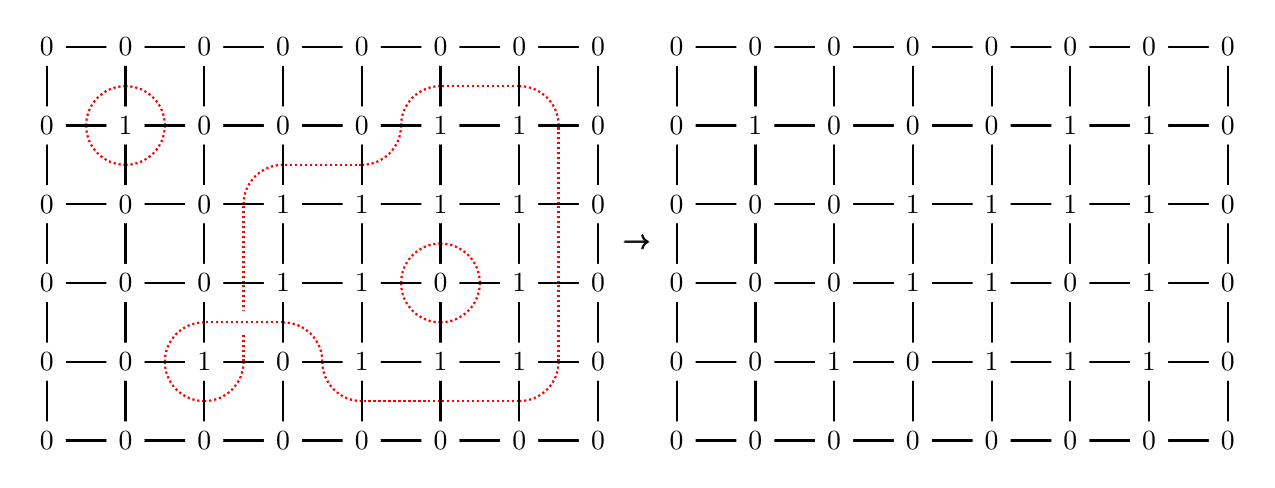
\begin{tikzpicture}
        % row1
        \cell{0}{0}{1}{1}
        \cellC{1}{0}{2}{1}
        \cellD{2}{0}{3}{1}
        \cellC{3}{0}{4}{1}
        \cellE{4}{0}{5}{1}
        \cellE{5}{0}{6}{1}
        \cellD{6}{0}{7}{1}
        % row2
        \cell{0}{1}{1}{2}
        \cellB{1}{1}{2}{2}
        \cellI{2}{1}{3}{2}
        \cellA{3}{1}{4}{2}
        \cellC{4}{1}{5}{2}
        \cellD{5}{1}{6}{2}
        \cellF{6}{1}{7}{2}
        % row3
        \cell{0}{2}{1}{3}
        \cell{1}{2}{2}{3}
        \cellF{2}{2}{3}{3}
        \cell{3}{2}{4}{3}
        \cellB{4}{2}{5}{3}
        \cellA{5}{2}{6}{3}
        \cellF{6}{2}{7}{3}
        % row4
        \cellC{0}{3}{1}{4}
        \cellD{1}{3}{2}{4}
        \cellB{2}{3}{3}{4}
        \cellE{3}{3}{4}{4}
        \cellD{4}{3}{5}{4}
        \cell{5}{3}{6}{4}
        \cellF{6}{3}{7}{4}
        % row5
        \cellB{0}{4}{1}{5}
        \cellA{1}{4}{2}{5}
        \cell{2}{4}{3}{5}
        \cell{3}{4}{4}{5}
        \cellB{4}{4}{5}{5}
        \cellE{5}{4}{6}{5}
        \cellA{6}{4}{7}{5}
        % label for row1
        \( \lablvertex{0}{0}{$0$} \)
        \( \lablvertex{1}{0}{$0$} \)
        \( \lablvertex{2}{0}{$0$} \)
        \( \lablvertex{3}{0}{$0$} \)
        \( \lablvertex{4}{0}{$0$} \)
        \( \lablvertex{5}{0}{$0$} \)
        \( \lablvertex{6}{0}{$0$} \)
        \( \lablvertex{7}{0}{$0$} \)
        % label for row1
        \( \lablvertex{0}{1}{$0$} \)
        \( \lablvertex{1}{1}{$0$} \)
        \( \lablvertex{2}{1}{$1$} \)
        \( \lablvertex{3}{1}{$0$} \)
        \( \lablvertex{4}{1}{$1$} \)
        \( \lablvertex{5}{1}{$1$} \)
        \( \lablvertex{6}{1}{$1$} \)
        \( \lablvertex{7}{1}{$0$} \)
        % label for row1
        \( \lablvertex{0}{2}{$0$} \)
        \( \lablvertex{1}{2}{$0$} \)
        \( \lablvertex{2}{2}{$0$} \)
        \( \lablvertex{3}{2}{$1$} \)
        \( \lablvertex{4}{2}{$1$} \)
        \( \lablvertex{5}{2}{$0$} \)
        \( \lablvertex{6}{2}{$1$} \)
        \( \lablvertex{7}{2}{$0$} \)
        % label for row1
        \( \lablvertex{0}{3}{$0$} \)
        \( \lablvertex{1}{3}{$0$} \)
        \( \lablvertex{2}{3}{$0$} \)
        \( \lablvertex{3}{3}{$1$} \)
        \( \lablvertex{4}{3}{$1$} \)
        \( \lablvertex{5}{3}{$1$} \)
        \( \lablvertex{6}{3}{$1$} \)
        \( \lablvertex{7}{3}{$0$} \)
        % label for row1
        \( \lablvertex{0}{4}{$0$} \)
        \( \lablvertex{1}{4}{$1$} \)
        \( \lablvertex{2}{4}{$0$} \)
        \( \lablvertex{3}{4}{$0$} \)
        \( \lablvertex{4}{4}{$0$} \)
        \( \lablvertex{5}{4}{$1$} \)
        \( \lablvertex{6}{4}{$1$} \)
        \( \lablvertex{7}{4}{$0$} \)
        % label for row1
        \( \lablvertex{0}{5}{$0$} \)
        \( \lablvertex{1}{5}{$0$} \)
        \( \lablvertex{2}{5}{$0$} \)
        \( \lablvertex{3}{5}{$0$} \)
        \( \lablvertex{4}{5}{$0$} \)
        \( \lablvertex{5}{5}{$0$} \)
        \( \lablvertex{6}{5}{$0$} \)
        \( \lablvertex{7}{5}{$0$} \)
        % arrow
        \( \lablnode{7.5}{2.5}{$\pmb{\to}$} \)

        % row1
        \cell{8}{0}{9}{1}
        \cell{9}{0}{10}{1}
        \cell{10}{0}{11}{1}
        \cell{11}{0}{12}{1}
        \cell{12}{0}{13}{1}
        \cell{13}{0}{14}{1}
        \cell{14}{0}{15}{1}
        % row2
        \cell{8}{1}{9}{2}
        \cell{9}{1}{10}{2}
        \cell{10}{1}{11}{2}
        \cell{11}{1}{12}{2}
        \cell{12}{1}{13}{2}
        \cell{13}{1}{14}{2}
        \cell{14}{1}{15}{2}
        % row3
        \cell{8}{2}{9}{3}
        \cell{9}{2}{10}{3}
        \cell{10}{2}{11}{3}
        \cell{11}{2}{12}{3}
        \cell{12}{2}{13}{3}
        \cell{13}{2}{14}{3}
        \cell{14}{2}{15}{3}
        % row4
        \cell{8}{3}{9}{4}
        \cell{9}{3}{10}{4}
        \cell{10}{3}{11}{4}
        \cell{11}{3}{12}{4}
        \cell{12}{3}{13}{4}
        \cell{13}{3}{14}{4}
        \cell{14}{3}{15}{4}
        % row5
        \cell{8}{4}{9}{5}
        \cell{9}{4}{10}{5}
        \cell{10}{4}{11}{5}
        \cell{11}{4}{12}{5}
        \cell{12}{4}{13}{5}
        \cell{13}{4}{14}{5}
        \cell{14}{4}{15}{5}

        % label for row1
        \( \lablvertex{8}{0}{$0$} \)
        \( \lablvertex{9}{0}{$0$} \)
        \( \lablvertex{10}{0}{$0$} \)
        \( \lablvertex{11}{0}{$0$} \)
        \( \lablvertex{12}{0}{$0$} \)
        \( \lablvertex{13}{0}{$0$} \)
        \( \lablvertex{14}{0}{$0$} \)
        \( \lablvertex{15}{0}{$0$} \)
        % label for row1
        \( \lablvertex{8}{1}{$0$} \)
        \( \lablvertex{9}{1}{$0$} \)
        \( \lablvertex{10}{1}{$1$} \)
        \( \lablvertex{11}{1}{$0$} \)
        \( \lablvertex{12}{1}{$1$} \)
        \( \lablvertex{13}{1}{$1$} \)
        \( \lablvertex{14}{1}{$1$} \)
        \( \lablvertex{15}{1}{$0$} \)
        % label for row1
        \( \lablvertex{8}{2}{$0$} \)
        \( \lablvertex{9}{2}{$0$} \)
        \( \lablvertex{10}{2}{$0$} \)
        \( \lablvertex{11}{2}{$1$} \)
        \( \lablvertex{12}{2}{$1$} \)
        \( \lablvertex{13}{2}{$0$} \)
        \( \lablvertex{14}{2}{$1$} \)
        \( \lablvertex{15}{2}{$0$} \)
        % label for row1
        \( \lablvertex{8}{3}{$0$} \)
        \( \lablvertex{9}{3}{$0$} \)
        \( \lablvertex{10}{3}{$0$} \)
        \( \lablvertex{11}{3}{$1$} \)
        \( \lablvertex{12}{3}{$1$} \)
        \( \lablvertex{13}{3}{$1$} \)
        \( \lablvertex{14}{3}{$1$} \)
        \( \lablvertex{15}{3}{$0$} \)
        % label for row1
        \( \lablvertex{8}{4}{$0$} \)
        \( \lablvertex{9}{4}{$1$} \)
        \( \lablvertex{10}{4}{$0$} \)
        \( \lablvertex{11}{4}{$0$} \)
        \( \lablvertex{12}{4}{$0$} \)
        \( \lablvertex{13}{4}{$1$} \)
        \( \lablvertex{14}{4}{$1$} \)
        \( \lablvertex{15}{4}{$0$} \)
        % label for row1
        \( \lablvertex{8}{5}{$0$} \)
        \( \lablvertex{9}{5}{$0$} \)
        \( \lablvertex{10}{5}{$0$} \)
        \( \lablvertex{11}{5}{$0$} \)
        \( \lablvertex{12}{5}{$0$} \)
        \( \lablvertex{13}{5}{$0$} \)
        \( \lablvertex{14}{5}{$0$} \)
        \( \lablvertex{15}{5}{$0$} \)

    \end{tikzpicture}
\end{center}

The critical point is this: even with the dotted lines removed, the vertex labeling uniquely identifies the polygon mosaic. This is true even if there are polygons surrounding other polygons. This is because the vertex labeling of an individual cell, which we will call a \textit{cell labeling}, uniquely corresponds with a cell $T_i$. This is shown below.

\begin{center}
    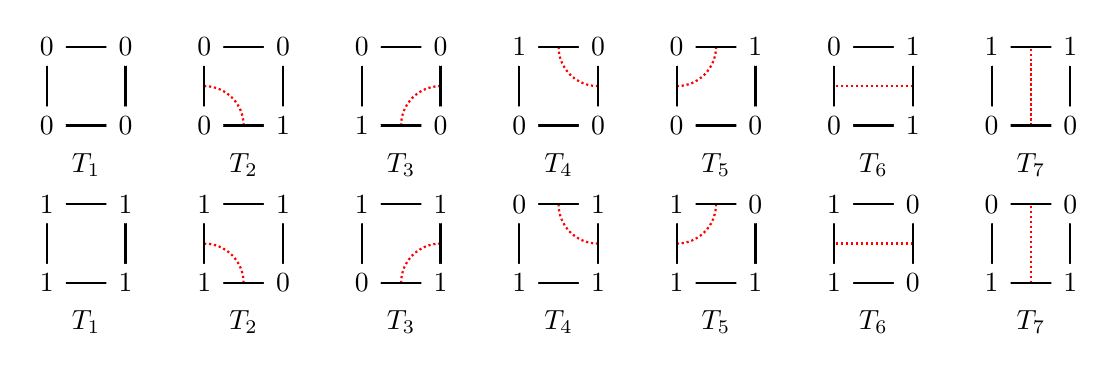
\begin{tikzpicture}
        % row 1
        \cell{-2}{0}{-1}{1}
        \( \lablnode{-1.5}{-0.5}{$T_1$} \) 
        \cellA{0}{0}{1}{1}
        \( \lablnode{0.5}{-0.5}{$T_2$} \) 
        \cellB{2}{0}{3}{1}
        \( \lablnode{2.5}{-0.5}{$T_3$} \) 
        \cellC{4}{0}{5}{1}
        \( \lablnode{4.5}{-0.5}{$T_4$} \) 
        \cellD{6}{0}{7}{1}
        \( \lablnode{6.5}{-0.5}{$T_5$} \) 
        \cellE{8}{0}{9}{1}
        \( \lablnode{8.5}{-0.5}{$T_6$} \) 
        \cellF{10}{0}{11}{1}
        \( \lablnode{10.5}{-0.5}{$T_7$} \) 

        \( \lablvertex{-2}{0}{$1$} \)
        \( \lablvertex{-2}{1}{$1$} \)
        \( \lablvertex{-1}{0}{$1$} \)
        \( \lablvertex{-1}{1}{$1$} \)

        \( \lablvertex{0}{0}{$1$} \)
        \( \lablvertex{0}{1}{$1$} \)
        \( \lablvertex{1}{0}{$0$} \)
        \( \lablvertex{1}{1}{$1$} \)

        \( \lablvertex{2}{0}{$0$} \)
        \( \lablvertex{2}{1}{$1$} \)
        \( \lablvertex{3}{0}{$1$} \)
        \( \lablvertex{3}{1}{$1$} \)

        \( \lablvertex{4}{0}{$1$} \)
        \( \lablvertex{4}{1}{$0$} \)
        \( \lablvertex{5}{0}{$1$} \)
        \( \lablvertex{5}{1}{$1$} \)

        \( \lablvertex{6}{0}{$1$} \)
        \( \lablvertex{6}{1}{$1$} \)
        \( \lablvertex{7}{0}{$1$} \)
        \( \lablvertex{7}{1}{$0$} \)

        \( \lablvertex{8}{0}{$1$} \)
        \( \lablvertex{8}{1}{$1$} \)
        \( \lablvertex{9}{0}{$0$} \)
        \( \lablvertex{9}{1}{$0$} \)

        \( \lablvertex{10}{0}{$1$} \)
        \( \lablvertex{10}{1}{$0$} \)
        \( \lablvertex{11}{0}{$1$} \)
        \( \lablvertex{11}{1}{$0$} \)


        % row 2
        \cell{-2}{2}{-1}{3}
        \( \lablnode{-1.5}{1.5}{$T_1$} \) 
        \cellA{0}{2}{1}{3}
        \( \lablnode{0.5}{1.5}{$T_2$} \) 
        \cellB{2}{2}{3}{3}
        \( \lablnode{2.5}{1.5}{$T_3$} \) 
        \cellC{4}{2}{5}{3}
        \( \lablnode{4.5}{1.5}{$T_4$} \) 
        \cellD{6}{2}{7}{3}
        \( \lablnode{6.5}{1.5}{$T_5$} \) 
        \cellE{8}{2}{9}{3}
        \( \lablnode{8.5}{1.5}{$T_6$} \) 
        \cellF{10}{2}{11}{3}
        \( \lablnode{10.5}{1.5}{$T_7$} \) 


        \( \lablvertex{-2}{2}{$0$} \)
        \( \lablvertex{-2}{3}{$0$} \)
        \( \lablvertex{-1}{2}{$0$} \)
        \( \lablvertex{-1}{3}{$0$} \)

        \( \lablvertex{0}{2}{$0$} \)
        \( \lablvertex{0}{3}{$0$} \)
        \( \lablvertex{1}{2}{$1$} \)
        \( \lablvertex{1}{3}{$0$} \)

        \( \lablvertex{2}{2}{$1$} \)
        \( \lablvertex{2}{3}{$0$} \)
        \( \lablvertex{3}{2}{$0$} \)
        \( \lablvertex{3}{3}{$0$} \)

        \( \lablvertex{4}{2}{$0$} \)
        \( \lablvertex{4}{3}{$1$} \)
        \( \lablvertex{5}{2}{$0$} \)
        \( \lablvertex{5}{3}{$0$} \)

        \( \lablvertex{6}{2}{$0$} \)
        \( \lablvertex{6}{3}{$0$} \)
        \( \lablvertex{7}{2}{$0$} \)
        \( \lablvertex{7}{3}{$1$} \)

        \( \lablvertex{8}{2}{$0$} \)
        \( \lablvertex{8}{3}{$0$} \)
        \( \lablvertex{9}{2}{$1$} \)
        \( \lablvertex{9}{3}{$1$} \)

        \( \lablvertex{10}{2}{$0$} \)
        \( \lablvertex{10}{3}{$1$} \)
        \( \lablvertex{11}{2}{$0$} \)
        \( \lablvertex{11}{3}{$1$} \)
    \end{tikzpicture}
\end{center}

We can then enumerate $p_{m,n}$ by enumerating the number of vertex labelings that correspond to a polygon mosaic. 

Consider the collection of vertex labelings for a $m \times n$ grid of cells. To correspond with a polygon mosaic, each boundary vertex is necessarily labeled $0$, and each interior vertex is labeled $0$ or $1$. Additionally, of these $2^{(m-1)(n-1)}$ labelings, the labelings that correspond with valid polygon mosaics are ones that do not contain the following two cell labelings.

\begin{center}
    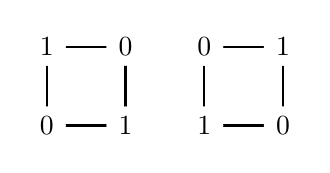
\begin{tikzpicture}
        % row1
        \cell{0}{0}{1}{1}
        \cell{2}{0}{3}{1}

        \( \lablvertex{0}{0}{$0$} \)
        \( \lablvertex{0}{1}{$1$} \)
        \( \lablvertex{1}{0}{$1$} \)
        \( \lablvertex{1}{1}{$0$} \)

        \( \lablvertex{2}{0}{$1$} \)
        \( \lablvertex{2}{1}{$0$} \)
        \( \lablvertex{3}{0}{$0$} \)
        \( \lablvertex{3}{1}{$1$} \)
        
    \end{tikzpicture}
\end{center}

These two cell labelings aren't associated with any of the cells $T_1, \dots, T_7$, and so cannot correspond with a polygon mosaic. We seek a recursive solution to enumerate the number of vertex labelings for an $m \times n$ grid with these  conditions: the labeling has a boundary of all $0$'s and does not contain the above cell labelings. 

Our solution accomplishes this by building $m \times n$ vertex labelings for fixed $m$ using vertex labelings of $m \times 1$ columns of cells. These columns have vertex labelings such that the top and bottom edge all labeled $0$. One of these columns for $m=3$ is below.

\begin{center}
    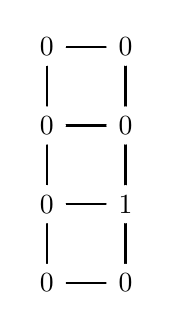
\begin{tikzpicture}
        \cell{0}{0}{1}{1}
        \cell{0}{1}{1}{2}
        \cell{0}{2}{1}{3}

        % col 1
        \( \lablvertex{0}{0}{$0$} \)
        \( \lablvertex{0}{1}{$0$} \)
        \( \lablvertex{0}{2}{$0$} \)
        \( \lablvertex{0}{3}{$0$} \)
        
        % col 2
        \( \lablvertex{1}{0}{$0$} \)
        \( \lablvertex{1}{1}{$1$} \)
        \( \lablvertex{1}{2}{$0$} \)
        \( \lablvertex{1}{3}{$0$} \)
        
        % index
        % \( \lablnode{0.5}{-1}{$(0,2)$} \)
    \end{tikzpicture}
\end{center}

It is useful to define an index for vertex labelings of these $m \times 1$ columns. To do this, consider reading a column of vertex labelings from bottom to top, ignoring the first and last $0$'s. If we interpret these sequences for the left and right column as binary numbers $b_{left}$ and $b_{right}$, the index in base ten is the pair $(b_{left}, b_{right})$. For example, for the above $m=3$ column, we have sequences $00$ for the left column and $10$ for the right column, so the index is $(0,2)$.

Next consider a column with index $(0, b_{1})$ for some $b_{1} \in [0,2^{m-1}-1]$. For reasons we will see later, let's call this the \textit{starting column}. Now consider appending a column with index $(b_{1}, b_{2})$ for some $b_{2} \in [0,2^{m-1}-1]$. For example, below is a diagram for appending our starting column $(0,2)$ with column $(2,3)$. 

\begin{center}
    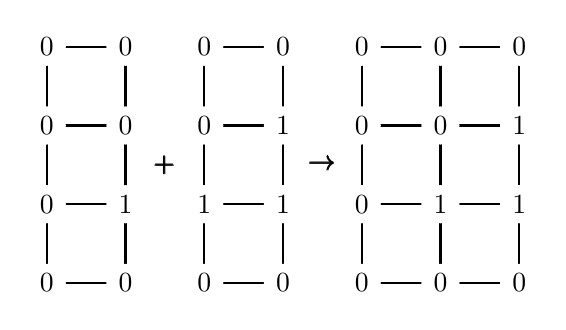
\begin{tikzpicture}
        \cell{0}{0}{1}{1}
        \cell{0}{1}{1}{2}
        \cell{0}{2}{1}{3}
        % col 1
        \( \lablvertex{0}{0}{$0$} \)
        \( \lablvertex{0}{1}{$0$} \)
        \( \lablvertex{0}{2}{$0$} \)
        \( \lablvertex{0}{3}{$0$} \)
        % col 2
        \( \lablvertex{1}{0}{$0$} \)
        \( \lablvertex{1}{1}{$1$} \)
        \( \lablvertex{1}{2}{$0$} \)
        \( \lablvertex{1}{3}{$0$} \)

        % plus
        \( \lablnode{1.5}{1.5}{$\pmb{+}$} \)

        \cell{2}{0}{3}{1}
        \cell{2}{1}{3}{2}
        \cell{2}{2}{3}{3}
        % col 1
        \( \lablvertex{2}{0}{$0$} \)
        \( \lablvertex{2}{1}{$1$} \)
        \( \lablvertex{2}{2}{$0$} \)
        \( \lablvertex{2}{3}{$0$} \)
        % col 1
        \( \lablvertex{3}{0}{$0$} \)
        \( \lablvertex{3}{1}{$1$} \)
        \( \lablvertex{3}{2}{$1$} \)
        \( \lablvertex{3}{3}{$0$} \)

        \( \lablnode{3.5}{1.5}{$\pmb{\to}$} \)

        \cell{4}{0}{5}{1}
        \cell{4}{1}{5}{2}
        \cell{4}{2}{5}{3}
        \cell{5}{0}{6}{1}
        \cell{5}{1}{6}{2}
        \cell{5}{2}{6}{3}

        % col 1
        \( \lablvertex{4}{0}{$0$} \)
        \( \lablvertex{4}{1}{$0$} \)
        \( \lablvertex{4}{2}{$0$} \)
        \( \lablvertex{4}{3}{$0$} \)
        % col 2
        \( \lablvertex{5}{0}{$0$} \)
        \( \lablvertex{5}{1}{$1$} \)
        \( \lablvertex{5}{2}{$0$} \)
        \( \lablvertex{5}{3}{$0$} \)
        % col 3
        \( \lablvertex{6}{0}{$0$} \)
        \( \lablvertex{6}{1}{$1$} \)
        \( \lablvertex{6}{2}{$1$} \)
        \( \lablvertex{6}{3}{$0$} \)


    \end{tikzpicture}
\end{center}

Notice that in the above example we have created a vertex labeling for an $m \times 2$ grid of cells, in which the left-most vertex column labels are all $0$ (left index of $0$). Also note that we did not create either illegal cell labelings with column $(2,3)$. However, we could append the column $(2,1)$, which would create an illegal cell labeling. 

Finally, if we further appended a column with label $(b_2,0)$, we would have created a vertex labeling with a boundary of all $0$'s. For this reason, let's call a column with index $(b,0)$ for $b \in [0,2^{m-1}-1]$ an \textit{ending column}. This vertex labeling would correspond with $1$ polygon mosaic if the middle column had index $(2,3)$, but not if the middle column had index $(2,1)$.

This motivates the creation of a matrix $A(m)$ to every column index $(i,j)$, where $A(m)_{i,j}=1$ if the column labeling corresponds with a legal polygon mosaic, and $0$ otherwise. For example, the $A(3)$ matrix corresponds with the following labeled columns. 

\begin{center}
    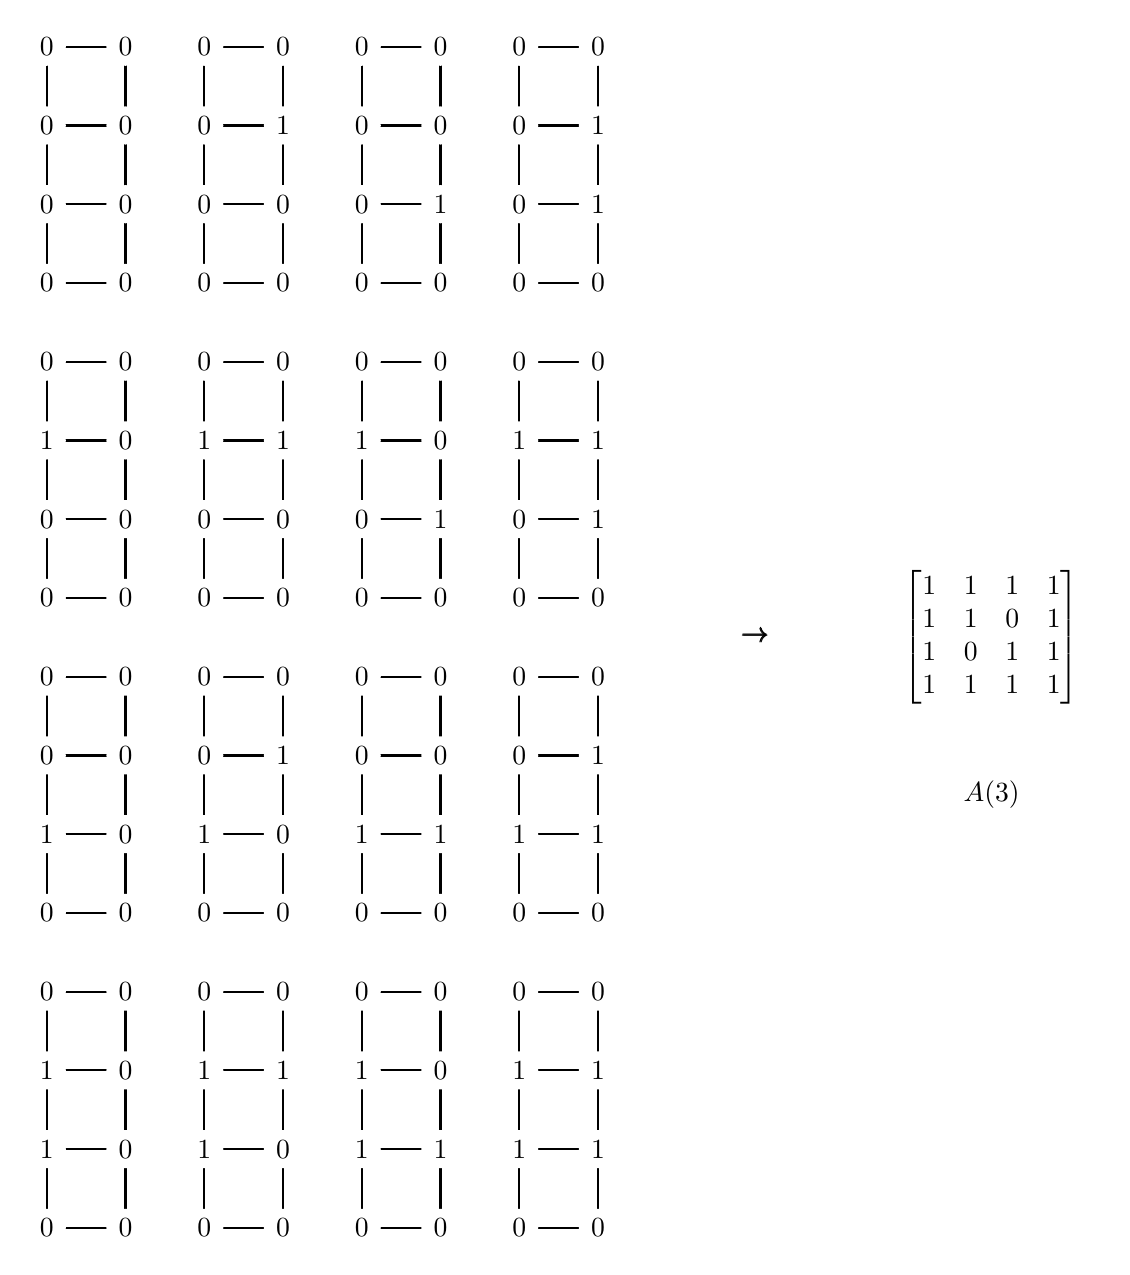
\begin{tikzpicture}
        % row1
        \cell{0}{0}{1}{1}
        \cell{0}{1}{1}{2}
        \cell{0}{2}{1}{3}

        \cell{2}{0}{3}{1}
        \cell{2}{1}{3}{2}
        \cell{2}{2}{3}{3}

        \cell{4}{0}{5}{1}
        \cell{4}{1}{5}{2}
        \cell{4}{2}{5}{3}

        \cell{6}{0}{7}{1}
        \cell{6}{1}{7}{2}
        \cell{6}{2}{7}{3}
        % row2
        \cell{0}{4}{1}{5}
        \cell{0}{5}{1}{6}
        \cell{0}{6}{1}{7}

        \cell{2}{4}{3}{5}
        \cell{2}{5}{3}{6}
        \cell{2}{6}{3}{7}

        \cell{4}{4}{5}{5}
        \cell{4}{5}{5}{6}
        \cell{4}{6}{5}{7}

        \cell{6}{4}{7}{5}
        \cell{6}{5}{7}{6}
        \cell{6}{6}{7}{7}
        % row3
        \cell{0}{8}{1}{9}
        \cell{0}{9}{1}{10}
        \cell{0}{10}{1}{11}

        \cell{2}{8}{3}{9}
        \cell{2}{9}{3}{10}
        \cell{2}{10}{3}{11}

        \cell{4}{8}{5}{9}
        \cell{4}{9}{5}{10}
        \cell{4}{10}{5}{11}

        \cell{6}{8}{7}{9}
        \cell{6}{9}{7}{10}
        \cell{6}{10}{7}{11}
        % row4
        \cell{0}{12}{1}{13}
        \cell{0}{13}{1}{14}
        \cell{0}{14}{1}{15}

        \cell{2}{12}{3}{13}
        \cell{2}{13}{3}{14}
        \cell{2}{14}{3}{15}

        \cell{4}{12}{5}{13}
        \cell{4}{13}{5}{14}
        \cell{4}{14}{5}{15}

        \cell{6}{12}{7}{13}
        \cell{6}{13}{7}{14}
        \cell{6}{14}{7}{15}
        % row 1
        \( \lablvertex{0}{0}{$0$} \)
        \( \lablvertex{0}{1}{$1$} \)
        \( \lablvertex{0}{2}{$1$} \)
        \( \lablvertex{0}{3}{$0$} \)
        
        \( \lablvertex{1}{0}{$0$} \)
        \( \lablvertex{1}{1}{$0$} \)
        \( \lablvertex{1}{2}{$0$} \)
        \( \lablvertex{1}{3}{$0$} \)
        
        \( \lablvertex{2}{0}{$0$} \)
        \( \lablvertex{2}{1}{$1$} \)
        \( \lablvertex{2}{2}{$1$} \)
        \( \lablvertex{2}{3}{$0$} \)
        
        \( \lablvertex{3}{0}{$0$} \)
        \( \lablvertex{3}{1}{$0$} \)
        \( \lablvertex{3}{2}{$1$} \)
        \( \lablvertex{3}{3}{$0$} \)
        
        \( \lablvertex{4}{0}{$0$} \)
        \( \lablvertex{4}{1}{$1$} \)
        \( \lablvertex{4}{2}{$1$} \)
        \( \lablvertex{4}{3}{$0$} \)
        
        \( \lablvertex{5}{0}{$0$} \)
        \( \lablvertex{5}{1}{$1$} \)
        \( \lablvertex{5}{2}{$0$} \)
        \( \lablvertex{5}{3}{$0$} \)
        
        \( \lablvertex{6}{0}{$0$} \)
        \( \lablvertex{6}{1}{$1$} \)
        \( \lablvertex{6}{2}{$1$} \)
        \( \lablvertex{6}{3}{$0$} \)
        
        \( \lablvertex{7}{0}{$0$} \)
        \( \lablvertex{7}{1}{$1$} \)
        \( \lablvertex{7}{2}{$1$} \)
        \( \lablvertex{7}{3}{$0$} \)
        % row 2
        \( \lablvertex{0}{4}{$0$} \)
        \( \lablvertex{0}{5}{$1$} \)
        \( \lablvertex{0}{6}{$0$} \)
        \( \lablvertex{0}{7}{$0$} \)
        
        \( \lablvertex{1}{4}{$0$} \)
        \( \lablvertex{1}{5}{$0$} \)
        \( \lablvertex{1}{6}{$0$} \)
        \( \lablvertex{1}{7}{$0$} \)
        
        \( \lablvertex{2}{4}{$0$} \)
        \( \lablvertex{2}{5}{$1$} \)
        \( \lablvertex{2}{6}{$0$} \)
        \( \lablvertex{2}{7}{$0$} \)
        
        \( \lablvertex{3}{4}{$0$} \)
        \( \lablvertex{3}{5}{$0$} \)
        \( \lablvertex{3}{6}{$1$} \)
        \( \lablvertex{3}{7}{$0$} \)
        
        \( \lablvertex{4}{4}{$0$} \)
        \( \lablvertex{4}{5}{$1$} \)
        \( \lablvertex{4}{6}{$0$} \)
        \( \lablvertex{4}{7}{$0$} \)
        
        \( \lablvertex{5}{4}{$0$} \)
        \( \lablvertex{5}{5}{$1$} \)
        \( \lablvertex{5}{6}{$0$} \)
        \( \lablvertex{5}{7}{$0$} \)
        
        \( \lablvertex{6}{4}{$0$} \)
        \( \lablvertex{6}{5}{$1$} \)
        \( \lablvertex{6}{6}{$0$} \)
        \( \lablvertex{6}{7}{$0$} \)
        
        \( \lablvertex{7}{4}{$0$} \)
        \( \lablvertex{7}{5}{$1$} \)
        \( \lablvertex{7}{6}{$1$} \)
        \( \lablvertex{7}{7}{$0$} \)
        % row 3
        \( \lablvertex{0}{8}{$0$} \)
        \( \lablvertex{0}{9}{$0$} \)
        \( \lablvertex{0}{10}{$1$} \)
        \( \lablvertex{0}{11}{$0$} \)
        
        \( \lablvertex{1}{8}{$0$} \)
        \( \lablvertex{1}{9}{$0$} \)
        \( \lablvertex{1}{10}{$0$} \)
        \( \lablvertex{1}{11}{$0$} \)
        
        \( \lablvertex{2}{8}{$0$} \)
        \( \lablvertex{2}{9}{$0$} \)
        \( \lablvertex{2}{10}{$1$} \)
        \( \lablvertex{2}{11}{$0$} \)
        
        \( \lablvertex{3}{8}{$0$} \)
        \( \lablvertex{3}{9}{$0$} \)
        \( \lablvertex{3}{10}{$1$} \)
        \( \lablvertex{3}{11}{$0$} \)
        
        \( \lablvertex{4}{8}{$0$} \)
        \( \lablvertex{4}{9}{$0$} \)
        \( \lablvertex{4}{10}{$1$} \)
        \( \lablvertex{4}{11}{$0$} \)
        
        \( \lablvertex{5}{8}{$0$} \)
        \( \lablvertex{5}{9}{$1$} \)
        \( \lablvertex{5}{10}{$0$} \)
        \( \lablvertex{5}{11}{$0$} \)
        
        \( \lablvertex{6}{8}{$0$} \)
        \( \lablvertex{6}{9}{$0$} \)
        \( \lablvertex{6}{10}{$1$} \)
        \( \lablvertex{6}{11}{$0$} \)
        
        \( \lablvertex{7}{8}{$0$} \)
        \( \lablvertex{7}{9}{$1$} \)
        \( \lablvertex{7}{10}{$1$} \)
        \( \lablvertex{7}{11}{$0$} \)
        % row 4
        \( \lablvertex{0}{12}{$0$} \)
        \( \lablvertex{0}{13}{$0$} \)
        \( \lablvertex{0}{14}{$0$} \)
        \( \lablvertex{0}{15}{$0$} \)
        
        \( \lablvertex{1}{12}{$0$} \)
        \( \lablvertex{1}{13}{$0$} \)
        \( \lablvertex{1}{14}{$0$} \)
        \( \lablvertex{1}{15}{$0$} \)
        
        \( \lablvertex{2}{12}{$0$} \)
        \( \lablvertex{2}{13}{$0$} \)
        \( \lablvertex{2}{14}{$0$} \)
        \( \lablvertex{2}{15}{$0$} \)
        
        \( \lablvertex{3}{12}{$0$} \)
        \( \lablvertex{3}{13}{$0$} \)
        \( \lablvertex{3}{14}{$1$} \)
        \( \lablvertex{3}{15}{$0$} \)
        
        \( \lablvertex{4}{12}{$0$} \)
        \( \lablvertex{4}{13}{$0$} \)
        \( \lablvertex{4}{14}{$0$} \)
        \( \lablvertex{4}{15}{$0$} \)
        
        \( \lablvertex{5}{12}{$0$} \)
        \( \lablvertex{5}{13}{$1$} \)
        \( \lablvertex{5}{14}{$0$} \)
        \( \lablvertex{5}{15}{$0$} \)
        
        \( \lablvertex{6}{12}{$0$} \)
        \( \lablvertex{6}{13}{$0$} \)
        \( \lablvertex{6}{14}{$0$} \)
        \( \lablvertex{6}{15}{$0$} \)
        
        \( \lablvertex{7}{12}{$0$} \)
        \( \lablvertex{7}{13}{$1$} \)
        \( \lablvertex{7}{14}{$1$} \)
        \( \lablvertex{7}{15}{$0$} \)

        % arrow
        \( \lablnode{9}{7.5}{$\pmb{\to}$} \)
        % matrix
        \( \lablnode{12}{7.5}{$\begin{bmatrix} 1 & 1 & 1 & 1 \\ 1 & 1 & 0 & 1 \\ 1 & 0 & 1 & 1 \\ 1 & 1 & 1 & 1 \end{bmatrix}$} \)

        \( \lablnode{12}{5.5}{$A(3)$} \)

    \end{tikzpicture}
\end{center}

$A(m)$ has the property that the $0$-th row represets all starting columns, and the $0$-th column represents all ending columns. Even more importantly, notice that $A(m)^2_{i,j}$ represents the number of $m \times 2$ grids with left-most index $i$ and right-most index $j$ that correspond with a legal polygon mosaic. In general, $(A(m)^n)_{i,j}$ represents this quantity for an $m \times n$ grid of cells, and so if we know $A(m)$ for some $m$, then $(A(m)^n)_{0,0} = p_{m,n}.$

The final component of the proof is constructing $A(m)$ for any $m$. Begin by  calculating $A(2)$ by identifying the number of legal polygon mosaics that correspond with each vertex coloring index $\{(0,0),(0,1),(1,0),(1,1)\}$, like so.

\begin{center}
    \begin{tikzpicture}
        % row1
        \cell{0}{0}{1}{1}
        \cell{0}{1}{1}{2}
        
        \cell{2}{0}{3}{1}
        \cell{2}{1}{3}{2}
        
        % row2
        \cell{0}{3}{1}{4}
        \cell{0}{4}{1}{5}
        
        \cell{2}{3}{3}{4}
        \cell{2}{4}{3}{5}
        % row 1
        \( \lablvertex{0}{0}{$0$} \)
        \( \lablvertex{0}{1}{$1$} \)
        \( \lablvertex{0}{2}{$0$} \)
        
        \( \lablvertex{1}{0}{$0$} \)
        \( \lablvertex{1}{1}{$0$} \)
        \( \lablvertex{1}{2}{$0$} \)
        
        \( \lablvertex{2}{0}{$0$} \)
        \( \lablvertex{2}{1}{$1$} \)
        \( \lablvertex{2}{2}{$0$} \)
        
        \( \lablvertex{3}{0}{$0$} \)
        \( \lablvertex{3}{1}{$1$} \)
        \( \lablvertex{3}{2}{$0$} \)
        % row 2
        \( \lablvertex{0}{3}{$0$} \)
        \( \lablvertex{0}{4}{$0$} \)
        \( \lablvertex{0}{5}{$0$} \)
        
        \( \lablvertex{1}{3}{$0$} \)
        \( \lablvertex{1}{4}{$0$} \)
        \( \lablvertex{1}{5}{$0$} \)
        
        \( \lablvertex{2}{3}{$0$} \)
        \( \lablvertex{2}{4}{$0$} \)
        \( \lablvertex{2}{5}{$0$} \)
        
        \( \lablvertex{3}{3}{$0$} \)
        \( \lablvertex{3}{4}{$1$} \)
        \( \lablvertex{3}{5}{$0$} \)

        % arrow
        \( \lablnode{5}{2.5}{$\pmb{\to}$} \)
        % matrix
        \( \lablnode{7}{2.5}{$\begin{bmatrix} 1 & 1 \\ 1 & 1 \end{bmatrix}$} \)

    \end{tikzpicture}
\end{center}

Next consider an arbitrary value $A(k)_{i,j}$ for any $k \geq 2$. This value is $1$ if the $k \times 1$ column with index $(i,j)$ can be part of a polygon mosaic, and $0$ otherwise. We can determine that specific values of $A(k+1)$ are multiples of $A(k)_{i,j}$ by considering the following operation on an arbitrary column with index $(i,j)$. Copy the column four times and replace the top two $0$'s of each column with the bottom row of labels from one of the four cell labelings below. 

\begin{center}
    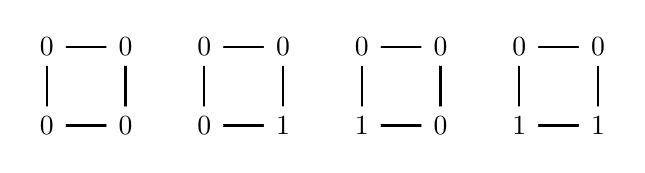
\begin{tikzpicture}
        % row1
        \cell{0}{0}{1}{1}
        \cell{2}{0}{3}{1}
        \cell{4}{0}{5}{1}
        \cell{6}{0}{7}{1}

        \( \lablvertex{0}{0}{$0$} \)
        \( \lablvertex{1}{0}{$0$} \)
        \( \lablvertex{2}{0}{$0$} \)
        \( \lablvertex{3}{0}{$1$} \)
        \( \lablvertex{4}{0}{$1$} \)
        \( \lablvertex{5}{0}{$0$} \)
        \( \lablvertex{6}{0}{$1$} \)
        \( \lablvertex{7}{0}{$1$} \)

        \( \lablvertex{0}{1}{$0$} \)
        \( \lablvertex{1}{1}{$0$} \)
        \( \lablvertex{2}{1}{$0$} \)
        \( \lablvertex{3}{1}{$0$} \)
        \( \lablvertex{4}{1}{$0$} \)
        \( \lablvertex{5}{1}{$0$} \)
        \( \lablvertex{6}{1}{$0$} \)
        \( \lablvertex{7}{1}{$0$} \)
        
    \end{tikzpicture}
\end{center}

For example, for the $m=2$ column with index $(0,1)$, this operation looks like the following.

\begin{center}
    \begin{tikzpicture}
        % row1
        \cell{-4.5}{2.5}{-3.5}{3.5}
        \cell{-4.5}{3.5}{-3.5}{4.5}

        % row 1
        \( \lablvertex{-4.5}{2.5}{$0$} \)
        \( \lablvertex{-4.5}{3.5}{$0$} \)
        \( \lablvertex{-4.5}{4.5}{$0$} \)
        
        \( \lablvertex{-3.5}{2.5}{$0$} \)
        \( \lablvertex{-3.5}{3.5}{$1$} \)
        \( \lablvertex{-3.5}{4.5}{$0$} \)

        % label
        \( \lablnode{-4}{1.5}{$A(2)_{0,1}$} \)

        % arrow
        \( \lablnode{-2}{3.5}{$\pmb{\to}$} \)

        % four columns
        \cell{0}{0}{1}{1}
        \cell{0}{1}{1}{2}
        \cell{0}{2}{1}{3}

        \cell{2}{0}{3}{1}
        \cell{2}{1}{3}{2}
        \cell{2}{2}{3}{3}

        \( \lablvertex{0}{0}{$0$} \)
        \( \lablvertex{0}{1}{$0$} \)
        \( \lablvertex{0}{2}{$1$} \)
        \( \lablvertex{0}{3}{$0$} \)
        
        \( \lablvertex{1}{0}{$0$} \)
        \( \lablvertex{1}{1}{$1$} \)
        \( \lablvertex{1}{2}{$0$} \)
        \( \lablvertex{1}{3}{$0$} \)
        
        \( \lablvertex{2}{0}{$0$} \)
        \( \lablvertex{2}{1}{$0$} \)
        \( \lablvertex{2}{2}{$1$} \)
        \( \lablvertex{2}{3}{$0$} \)
        
        \( \lablvertex{3}{0}{$0$} \)
        \( \lablvertex{3}{1}{$1$} \)
        \( \lablvertex{3}{2}{$1$} \)
        \( \lablvertex{3}{3}{$0$} \)
        
        \cell{0}{4}{1}{5}
        \cell{0}{5}{1}{6}
        \cell{0}{6}{1}{7}
        
        \cell{2}{4}{3}{5}
        \cell{2}{5}{3}{6}
        \cell{2}{6}{3}{7}

        \( \lablvertex{0}{4}{$0$} \)
        \( \lablvertex{0}{5}{$0$} \)
        \( \lablvertex{0}{6}{$0$} \)
        \( \lablvertex{0}{7}{$0$} \)
        
        \( \lablvertex{1}{4}{$0$} \)
        \( \lablvertex{1}{5}{$1$} \)
        \( \lablvertex{1}{6}{$0$} \)
        \( \lablvertex{1}{7}{$0$} \)
        
        \( \lablvertex{2}{4}{$0$} \)
        \( \lablvertex{2}{5}{$0$} \)
        \( \lablvertex{2}{6}{$0$} \)
        \( \lablvertex{2}{7}{$0$} \)
        
        \( \lablvertex{3}{4}{$0$} \)
        \( \lablvertex{3}{5}{$1$} \)
        \( \lablvertex{3}{6}{$1$} \)
        \( \lablvertex{3}{7}{$0$} \)

        \( \lablnode{5}{3.5}{$\pmb{\to}$} \)

        \( \lablnode{7.5}{3.5}{$\begin{bmatrix} A(3)_{0,2} & A(3)_{0,3} \\ A(3)_{1,2} & A(3)_{1,3} \end{bmatrix}$} \)

    \end{tikzpicture}
\end{center}

This operation results in $4$ new columns that are represented in $A(k+1)$. In our example, specifically we get the following. 

$$
\begin{bmatrix} 
    A(3)_{0,2} & A(3)_{0,3} \\ 
    A(3)_{1,2} & A(3)_{1,3} 
\end{bmatrix} = 
\begin{bmatrix} 
    1A(2)_{i,j} & 1A(2)_{i,j} \\ 
    0A(2)_{i,j} & 1A(2)_{i,j} 
\end{bmatrix},
$$

Critically, this transformation \textit{only} changes the identity of the top two tiles. This implies that the same value coefficients computed by comparing $A(2)$ and $A(3)$ can be used for any $m \times 1$ column, as long as both column indices $(i,j)$ are congruent $\text{mod } 2$. Furthermore, if one writes $A(k)$ as the block matrix

$$A(k) = \begin{bmatrix} A_{0,0} & A_{0,1} \\ A_{1,0} & A_{1,1} \end{bmatrix},$$

where $A_{\hat{i},\hat{j}} \in \mathbb{R}^{2^{k-2} \times 2^{k-2}}$, then all column's represented in $A_{\hat{i},\hat{j}}$ have indices $(i,j) \equiv (\hat{i},\hat{j}) \text{ mod } 2$. This allows us to write that in general, if $A(k) = \begin{bmatrix} A_{0,0} & A_{0,1} \\ A_{1,0} & A_{1,1} \end{bmatrix},$
then

\begin{equation}\label{eqn: coefficient matrix prod}
    \begin{bmatrix}
        V_{0,0}A_{0,0} & V_{0,1}A_{0,0} & V_{0,2}A_{0,1} & V_{0,3}A_{0,1} \\
        V_{1,0}A_{0,0} & V_{1,1}A_{0,0} & V_{1,2}A_{0,1} & V_{1,3}A_{0,1} \\
        V_{2,0}A_{1,0} & V_{2,1}A_{1,0} & V_{2,2}A_{1,1} & V_{2,3}A_{1,1} \\
        V_{3,0}A_{1,0} & V_{3,1}A_{1,0} & V_{3,2}A_{1,1} & V_{3,3}A_{1,1} \\
    \end{bmatrix}.
\end{equation}


where $V \in \mathbb{R}^{4 \times 4}$ can be found after directly computing $A(2)$ and $A(3)$, then solving the following equation.

$$
\begin{bmatrix}
    A(3)_{0,0} & A(3)_{0,1} & A(3)_{0,2} & A(3)_{0,3} \\
    A(3)_{1,0} & A(3)_{1,1} & A(3)_{1,2} & A(3)_{1,3} \\
    A(3)_{2,0} & A(3)_{2,1} & A(3)_{2,2} & A(3)_{2,3} \\
    A(3)_{3,0} & A(3)_{3,1} & A(3)_{3,2} & A(3)_{3,3} \\
\end{bmatrix} = 
\begin{bmatrix}
    V_{0,0}A(2)_{0,0} & V_{0,1}A(2)_{0,0} & V_{0,2}A(2)_{0,1} & V_{0,3}A(2)_{0,1} \\
    V_{1,0}A(2)_{0,0} & V_{1,1}A(2)_{0,0} & V_{1,2}A(2)_{0,1} & V_{1,3}A(2)_{0,1} \\
    V_{2,0}A(2)_{1,0} & V_{2,1}A(2)_{1,0} & V_{2,2}A(2)_{1,1} & V_{2,3}A(2)_{1,1} \\
    V_{3,0}A(2)_{1,0} & V_{3,1}A(2)_{1,0} & V_{3,2}A(2)_{1,1} & V_{3,3}A(2)_{1,1} \\
\end{bmatrix}
$$

This is solved by

$$V = 
\begin{bmatrix} 
    1 & 1 & 1 & 1 \\ 
    1 & 1 & 0 & 1 \\ 
    1 & 0 & 1 & 1 \\ 
    1 & 1 & 1 & 1 
\end{bmatrix}
$$


which completes the proof.

\end{proof}

The method detailed in Theorem \ref{thm: main theorem} generalizes to other tile sets, which we tabularize in Section \ref{section: summary of results} without proof. Interestingly, the method not only generalizes to other tile sets, but can also be augmented to enumerate the more complicated ``messy" polygon mosaics.



As demonstrated in the proof of Theorem \ref{thm: messy mosaics}, the enumeration of both polygon mosaics and mosaics that do not contain a polygon share the same structure, and only differ by the identity of the matrices $A(2), V$. We summarize these matrices for various collections of tiles below.

\begin{center}
    \begin{tblr}{
  colspec = {X[c,h]X[c]X[c]X[c]},
  stretch = 0,
  rowsep = 6pt,
  hlines = {black, 1pt},
  vlines = {black, 1pt},
}
  \textbf{Tile Set} & \textbf{Polygon Mosaics} & \textbf{Messy Polygon Mosaics}\\
  
  \resizebox{0.3\textwidth}{!}{%
  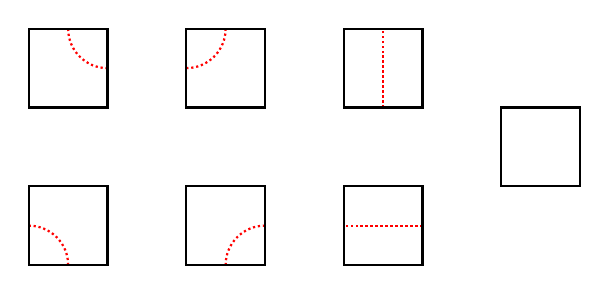
\begin{tikzpicture}
      \cellA{0}{0}{1}{1}
      \cellB{2}{0}{3}{1}
      \cellC{0}{2}{1}{3}
      \cellD{2}{2}{3}{3}
      
      \cellE{4}{0}{5}{1}
      \cellF{4}{2}{5}{3}

      \cell{6}{1}{7}{2}

    \end{tikzpicture}
    } 
    & 
    $\begin{bmatrix}
    1 & 1 \\
    1 & 1
    \end{bmatrix},
    \begin{bmatrix} 
    1 & 1 & 1 & 1 \\ 
    1 & 1 & 0 & 1 \\ 
    1 & 0 & 1 & 1 \\ 
    1 & 1 & 1 & 1 
    \end{bmatrix}$
    & 
    $\begin{bmatrix}
        7^2 & 1 \\
        -1 & 1
    \end{bmatrix},
    \begin{bmatrix}
        7 & \frac{1}{7} & 7 & 1 \\
        -\frac{1}{7} & 1 & 0 & 1 \\
        7 & 0 & 7  & 1 \\
        1 & -1 & 1 & 7 \\
    \end{bmatrix}$
    \\
    
    \resizebox{0.3\textwidth}{!}{%
    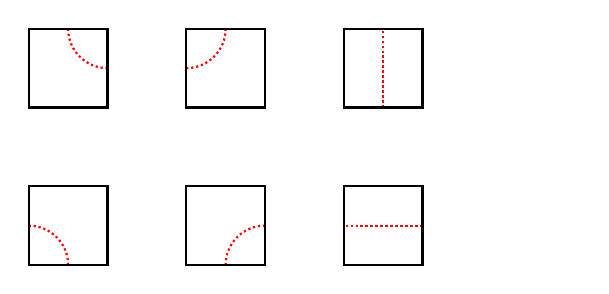
\begin{tikzpicture}
        \cellA{0}{0}{1}{1}
        \cellB{2}{0}{3}{1}
        \cellC{0}{2}{1}{3}
        \cellD{2}{2}{3}{3}
        
        \cellE{4}{0}{5}{1}
        \cellF{4}{2}{5}{3}
        % invisible cell for spacing
        \spacecell{6}{1}{7}{2}
    \end{tikzpicture}
    } 
    & 
    TODO 
    & 
    $\begin{bmatrix}
        6^2 & 1 \\
        -1 & 1
    \end{bmatrix},
    \begin{bmatrix}
        6 & \frac{1}{6} & 6 & 1 \\
        -\frac{1}{6} & 1 & 0 & 1 \\
        6 & 0 & 6  & 1 \\
        1 & -1 & 1 & 6 \\
    \end{bmatrix}$ 
    \\

    \resizebox{0.3\textwidth}{!}{%
    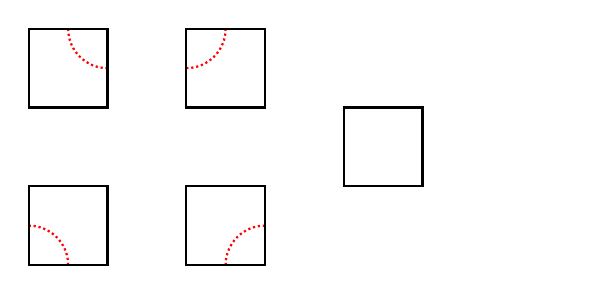
\begin{tikzpicture}
        \cellA{0}{0}{1}{1}
        \cellB{2}{0}{3}{1}
        \cellC{0}{2}{1}{3}
        \cellD{2}{2}{3}{3}
        
        \cell{4}{1}{5}{2}
        % invisible cell for spacing
        \spacecell{6}{1}{7}{2}
        
    \end{tikzpicture}
    } 
    & 
    $\begin{bmatrix}
        1 & 1 \\
        1 & 0
    \end{bmatrix}$, TODO 
    & 
    TODO
    \\

    \resizebox{0.3\textwidth}{!}{%
    \begin{tikzpicture}
        \cellA{0}{0}{1}{1}
        \cellB{2}{0}{3}{1}
        \cellC{0}{2}{1}{3}
        \cellD{2}{2}{3}{3}
        % invisible cell for spacing
        \spacecell{4}{1}{5}{2}
        % invisible cell for spacing
        \spacecell{6}{1}{7}{2}
    \end{tikzpicture}
      } 
    & 
    TODO
    & 
    TODO 
    \\
  
\end{tblr}
\end{center}


\begin{theorem}
    \label{thm: growth rate}    
    Let the probability that an $(m,n)$-mosaic \textit{does not} contain a SAP be denoted $p_{m,n} = \frac{t_{m,n}}{7^{nm}}$. Then the growth rate of the main diagonal $p_{n,n}$ has
    $$\gamma = \lim_{n \to \infty} \frac{p_{n+1,n+1}p_{n-1,n-1}}{p_{n,n}^2} = ?$$
\end{theorem}


\section{Introduction}

Consider the following $6$ unit squares with markings on them.

%figure of tiles (colored marknigs!)
\begin{center}
    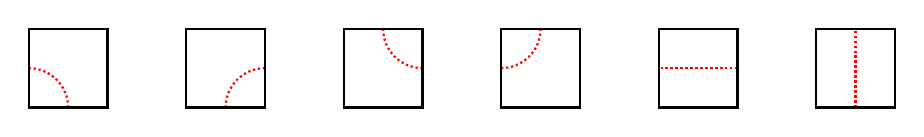
\begin{tikzpicture}
    \cellA{0}{0}{1}{1}
    \cellB{2}{0}{3}{1}
    \cellC{4}{0}{5}{1}
    \cellD{6}{0}{7}{1}
    \cellE{8}{0}{9}{1}
    \cellF{10}{0}{11}{1}    
    \end{tikzpicture}
\end{center}

Call these squares \textit{tiles}. 

\begin{definition}
An $(n,m)$-\textit{mosaic} is a rectangular grid made up of tiles.
\end{definition}

\begin{exmp}
An example of a $(7,5)$-mosaic:
\begin{center}
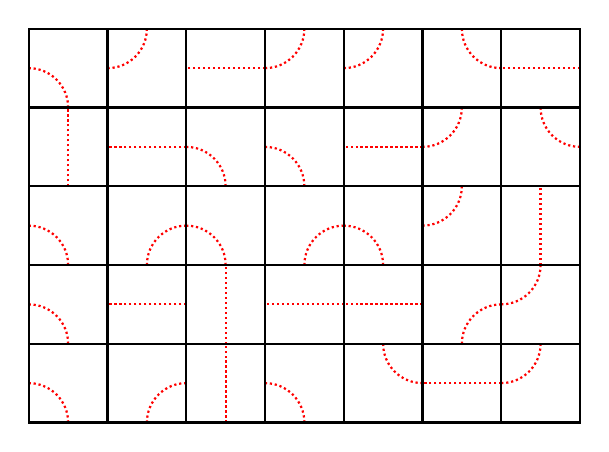
\begin{tikzpicture}
% row1
\cellA{0}{0}{1}{1}
\cellB{1}{0}{2}{1}
\cellF{2}{0}{3}{1}
\cellA{3}{0}{4}{1}
\cellC{4}{0}{5}{1}
\cellE{5}{0}{6}{1}
\cellD{6}{0}{7}{1}
% row2
\cellA{0}{1}{1}{2}
\cellE{1}{1}{2}{2}
\cellF{2}{1}{3}{2}
\cellE{3}{1}{4}{2}
\cellE{4}{1}{5}{2}
\cellB{5}{1}{6}{2}
\cellD{6}{1}{7}{2}
% row3
\cellA{0}{2}{1}{3}
\cellB{1}{2}{2}{3}
\cellA{2}{2}{3}{3}
\cellB{3}{2}{4}{3}
\cellA{4}{2}{5}{3}
\cellD{5}{2}{6}{3}
\cellF{6}{2}{7}{3}
% row4
\cellF{0}{3}{1}{4}
\cellE{1}{3}{2}{4}
\cellA{2}{3}{3}{4}
\cellA{3}{3}{4}{4}
\cellE{4}{3}{5}{4}
\cellD{5}{3}{6}{4}
\cellC{6}{3}{7}{4}
% row5
\cellA{0}{4}{1}{5}
\cellD{1}{4}{2}{5}
\cellE{2}{4}{3}{5}
\cellD{3}{4}{4}{5}
\cellD{4}{4}{5}{5}
\cellC{5}{4}{6}{5}
\cellE{6}{4}{7}{5}
\end{tikzpicture}
\end{center}
\end{exmp}

Clearly there are $6^{nm}$ possible mosaics. Which of these mosaics contain self-avoiding polygons?

%example of a mosaic with an enclosed region
\begin{exmp}
An example of a $(7,5)$-mosaic with a self-avoiding polygon:
\begin{center}
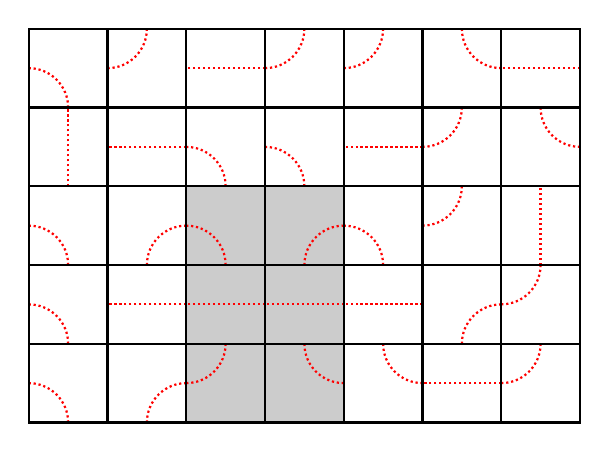
\begin{tikzpicture}
% row1
\cellA{0}{0}{1}{1}
\cellB{1}{0}{2}{1}
\cellDf{2}{0}{3}{1}
\cellCf{3}{0}{4}{1}
\cellC{4}{0}{5}{1}
\cellE{5}{0}{6}{1}
\cellD{6}{0}{7}{1}
% row2
\cellA{0}{1}{1}{2}
\cellE{1}{1}{2}{2}
\cellEf{2}{1}{3}{2}
\cellEf{3}{1}{4}{2}
\cellE{4}{1}{5}{2}
\cellB{5}{1}{6}{2}
\cellD{6}{1}{7}{2}
% row3
\cellA{0}{2}{1}{3}
\cellB{1}{2}{2}{3}
\cellAf{2}{2}{3}{3}
\cellBf{3}{2}{4}{3}
\cellA{4}{2}{5}{3}
\cellD{5}{2}{6}{3}
\cellF{6}{2}{7}{3}
% row4
\cellF{0}{3}{1}{4}
\cellE{1}{3}{2}{4}
\cellA{2}{3}{3}{4}
\cellA{3}{3}{4}{4}
\cellE{4}{3}{5}{4}
\cellD{5}{3}{6}{4}
\cellC{6}{3}{7}{4}
% row5
\cellA{0}{4}{1}{5}
\cellD{1}{4}{2}{5}
\cellE{2}{4}{3}{5}
\cellD{3}{4}{4}{5}
\cellD{4}{4}{5}{5}
\cellC{5}{4}{6}{5}
\cellE{6}{4}{7}{5}
\end{tikzpicture}
\end{center}
\end{exmp}

Let $t_{n,m}$ be the number of mosaics that have at least one self avoiding polygon (SAP). From the fact that the smallest SAP is

\begin{center}
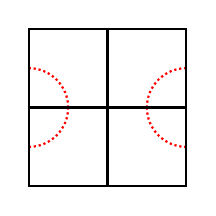
\begin{tikzpicture}

% row1
\cellD{0}{0}{1}{1}
\cellC{1}{0}{2}{1}
% row2
\cellA{0}{1}{1}{2}
\cellB{1}{1}{2}{2}
\end{tikzpicture}
\end{center}

we have that $t_{n,1}=t_{1,m}=0$, and $t_{2,2} = 1$. What else can be said?

\begin{theorem}\label{thm: m=2 case}
Setting $m=2$ gives
\begin{equation}
    T_2(x) = \sum_{n \geq 2}t_{n,2}x^n = \frac{x^2}{(1-36x)(1-37x+37x^2)}.
\end{equation}
This can be solved for $n \geq 2$ to give
\begin{equation}
     t_{n,2}= 6^{2n} - \frac{1}{\beta-\alpha}((36\beta-35)\beta^{-n+1} - (36\alpha - 35)\alpha^{-n+1})
\end{equation}

where $\alpha = \frac{1}{2} + \frac{1}{2}\sqrt{\frac{33}{37}}$ and $\beta = \frac{1}{2} - \frac{1}{2}\sqrt{\frac{33}{37}}$.
\end{theorem}

\begin{proof}
We prove that $t_{n,2}$ has
$$t_{n,2} = 36t_{n-1,2} + \sum_{i=2}^{n}(6^{2(n-i)}-t_{n-i,2}).$$

Split $t_{n,2}$ into $S_n$ and $S_n^c$. $S_n$ contains the mosaics that have just $1$ SAP that contains the left-most two cells. This means $S_n^c$ contains all mosaics that contain multiple SAPs and mosaics that contain only $1$ SAP, but that does not contain the two left-most cells.

The subset $S_n$ can be split further by the length of each SAP $i$. 

\begin{center}
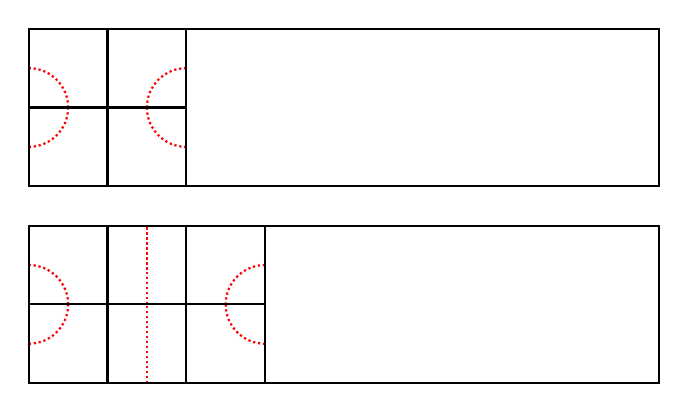
\begin{tikzpicture}\label{fig: S breakdown}
\draw[thick] ( 0 , 0 ) rectangle ( 8 , 2 );
% row1
\cellD{0}{0}{1}{1}
\cellC{1}{0}{2}{1}
% row2
\cellA{0}{1}{1}{2}
\cellB{1}{1}{2}{2}

\draw[thick] ( 0 , -2.5 ) rectangle ( 8 , -0.5 );
% row1
\cellD{0}{-2.5}{1}{-1.5}
\cellF{1}{-2.5}{2}{-1.5}
\cellC{2}{-2.5}{3}{-1.5}
% row2
\cellA{0}{-1.5}{1}{-0.5}
\cellF{1}{-1.5}{2}{-0.5}
\cellB{2}{-1.5}{3}{-0.5}

\end{tikzpicture}
\captionof{figure}{Members of $S_n$ of lengths $i=2$ and $i=3$}
\end{center}

As $S_n$ counts the number of mosaics that only contain $1$ SAP, the blank space in Figure \ref{fig: S breakdown} must have no SAPs. The number of mosaics that have no SAPs is $6^{2(n-i)}-t_{n-i,2}$. As a SAP's width can range from $2$ to $n$, we have $|S_n| = \sum_{i=2}^{n}(6^{2(n-i)}-t_{n-i,2}).$

Now consider $S_n^c$. The mosaics that belong to this set can be represented by the following diagram,

\begin{center}
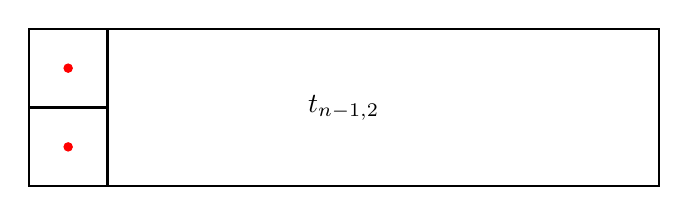
\begin{tikzpicture}
\draw[thick] ( 0 , 0 ) rectangle ( 8 , 2 );
% row1
\cellopen{0}{0}{1}{1}
% row2
\cellopen{0}{1}{1}{2}
% text
\node[shape=circle,draw=white,fill=white, inner sep=0pt,minimum size=0pt] (A) at ( 4 , 1 ){$t_{n-1,2}$};
\end{tikzpicture}
\captionof{figure}{Representation of $S_n^c$}\label{fig: Sc breakdown}
\end{center}

where the red dot in the left most cells indicate any marking. For this paper, we will refer to a cell that can have any marking as an \textit{open}. We can conclude that $|S_n^c| = 6^{2}t_{n-1,2}$. Combining $S_n$ and $S_n^c$ gives the recurrence relation. Standard techniques then give the generating function and formula.
\end{proof}

\begin{theorem}\label{thm: m=3 case}
Setting $m=3$ gives
\begin{equation}
    T_3(x) = \sum_{n \geq 2}t_{n,3}x^n = \frac{(73-414x)x^2}{(1-216x)(1-228x+2699x^2-7758x^3)}
\end{equation}
\end{theorem}

\begin{proof}
For $t_{n,3}$ we directly compute the generating function $T_3(x)=\sum_{n \geq 2}t_{n,3}x^n$ using the following recurrence relation
$$t_{3,n} = 6^3 t_{n-1,3} + \sum_{i = 2}^{n}(6^{3(n-i)} - t_{n-i,3})f_{i},$$
where $f_{i}$ is the number of mosaics in an $i \times 3$ grid  that contain just one SAP that has cells in the left-most column. We similarly split $t_{n,3}$ into $S_n$ and $S_n^c$. Here let $S_n$ be the set that contains the mosaics that have just $1$ SAP that has cells in the left-most column. Therefore $S_n^c$ contains all mosaics that contain multiple SAPs and mosaics that contain $1$ SAP that does not have cells in the left-most column. 

Similarly for the $n=2$ case, $S_n^c$ can be easily enumerated. 
\begin{center}
    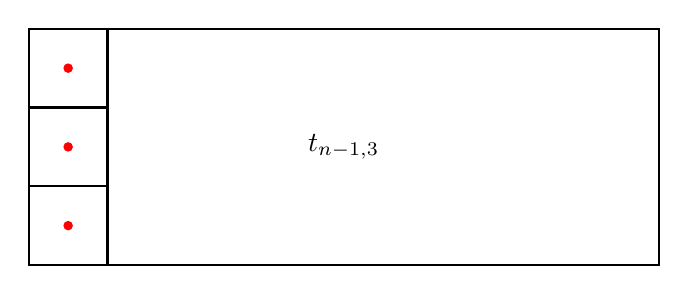
\begin{tikzpicture}
    \draw[thick] ( 0 , 0 ) rectangle ( 8 , 3 );
    % row1
    \cellopen{0}{0}{1}{1}
    % row2
    \cellopen{0}{1}{1}{2}
    % row3
    \cellopen{0}{2}{1}{3}
    % text
    \node[shape=circle,draw=white,fill=white, inner sep=0pt,minimum size=0pt] (A) at ( 4 , 1.5 ){$t_{n-1,3}$};
    \end{tikzpicture}
    \captionof{figure}{Representation of $S_n^c$}\label{fig: Sc breakdown for 3}
\end{center}

It is clear to see that $|S_n^c| = 6^3 t_{n-1,3},$ and so 
$$\sum_{n \geq 2} |S_n^c|x^n = 6^3 xT(x).$$

To enumerate $S_n$, as in the $n=2$ case, the SAP starts in the first column and ends at column $i$, after which there are no SAPs. This allows us to conclude that $|S_n| = \sum_{i = 2}^{n}(6^{3(n-i)} - t_{n-i,3})f_{i},$, where $f_i$ is the number of ways the cells to the left of and including column $i$ can contain $1$ SAP that includes the left-most column. To find the identity of $f_i$, we study the $4$ cases below.

\begin{center}
    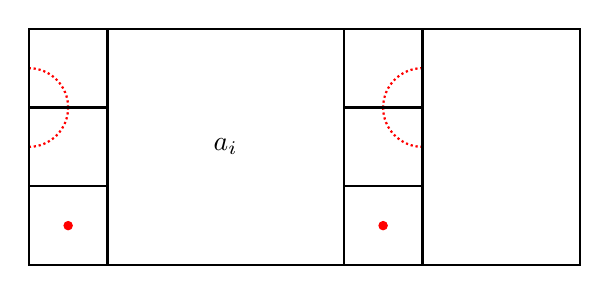
\begin{tikzpicture}
        \draw[thick] ( 0 , 0 ) rectangle ( 7 , 3 );
        % row1
        \cellopen{0}{0}{1}{1}
        % row2
        \cellD{0}{1}{1}{2}
        % row3
        \cellA{0}{2}{1}{3}

        % row1
        \cellopen{4}{0}{5}{1}
        % row2
        \cellC{4}{1}{5}{2}
        % row3
        \cellB{4}{2}{5}{3}

        % text
        \node[shape=circle,draw=white,fill=white, inner sep=0pt,minimum size=0pt] (A) at ( 2.5 , 1.5 ){$a_{i}$};
    \end{tikzpicture}
    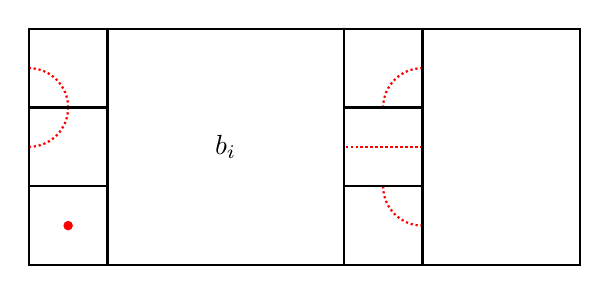
\begin{tikzpicture}
        \draw[thick] ( 0 , 0 ) rectangle ( 7 , 3 );
        % row1
        \cellopen{0}{0}{1}{1}
        % row2
        \cellD{0}{1}{1}{2}
        % row3
        \cellA{0}{2}{1}{3}

        % row1
        \cellC{4}{0}{5}{1}
        % row2
        \cellE{4}{1}{5}{2}
        % row3
        \cellB{4}{2}{5}{3}

        % text
        \node[shape=circle,draw=white,fill=white, inner sep=0pt,minimum size=0pt] (A) at ( 2.5 , 1.5 ){$b_{i}$};
    \end{tikzpicture}
\end{center}
\begin{center}
    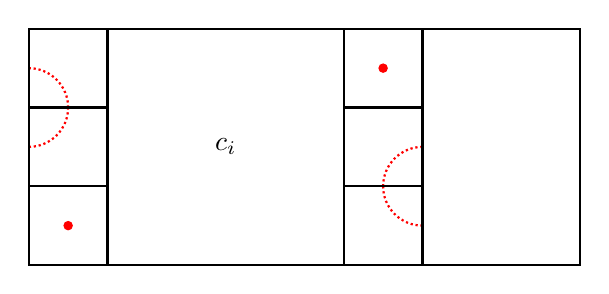
\begin{tikzpicture}
        \draw[thick] ( 0 , 0 ) rectangle ( 7 , 3 );
        % row1
        \cellopen{0}{0}{1}{1}
        % row2
        \cellD{0}{1}{1}{2}
        % row3
        \cellA{0}{2}{1}{3}

        % row1
        \cellC{4}{0}{5}{1}
        % row2
        \cellB{4}{1}{5}{2}
        % row3
        \cellopen{4}{2}{5}{3}

        % text
        \node[shape=circle,draw=white,fill=white, inner sep=0pt,minimum size=0pt] (A) at ( 2.5 , 1.5 ){$c_{i}$};
    \end{tikzpicture}
    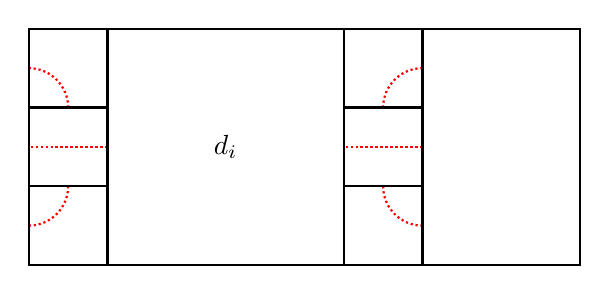
\begin{tikzpicture}
        \draw[thick] ( 0 , 0 ) rectangle ( 7 , 3 );
        % row1
        \cellD{0}{0}{1}{1}
        % row2
        \cellE{0}{1}{1}{2}
        % row3
        \cellA{0}{2}{1}{3}

        % row1
        \cellC{4}{0}{5}{1}
        % row2
        \cellE{4}{1}{5}{2}
        % row3
        \cellB{4}{2}{5}{3}

        % text
        \node[shape=circle,draw=white,fill=white, inner sep=0pt,minimum size=0pt] (A) at ( 2.5 , 1.5 ){$d_{i}$};
    \end{tikzpicture}
\end{center}

It is easy to see that $a_2 = 36$ and $a_3 = 216$. As $i$ increases, one can see that the enumeration of $a_i$ is related to smaller values of $a_i$ and $b_i$, more specifically
$$a_i = 6a_{i-1} + 6^2 b_{i-2}.$$

We find similar relations with the other $3$ cases, namely
$$b_n = 6b_{n-1} + 6^2 d_{n-2}$$
where $b_2 = 0$ and $b_3 = 6$
$$c_n = 6c_{n-1} + 6^2 b_{n-2}$$
where $c_2 = 0$ and $c_3 = 0$
$$d_n = 6d_{n-1} + 6^2 b_{n-2}$$
where $d_2 = 1$ and $d_3 = 6.$

Combining these $4$ cases, and accounting for the appropriate symmetries, we arrive at

$$f_i = 2a_i + 4b_i + 2c_i + d_i.$$

Solving this series of recurrence relations using generating functions gives

$$F(x) = \sum_{i \geq 2} f_i x^i = \frac{73 - 414x}{1-12x+43x^2}$$

This allows us to write 
$$\sum_{n \geq 2} |S_n|x^n = \left(\frac{1}{1-6^3x}-T(x)\right)F(x).$$

Combining these two generating functions and simplifying gives the result.

\end{proof}

\section{Full Solution}

TODO writeup, credit Farstar31!

$$
M(2) = \begin{bmatrix}
36 & 1 \\
-1 & 1
\end{bmatrix}
$$

For $h \geq 2$, then if
$$
M(h) = \begin{bmatrix}
M_1 & M_2 \\
M_3 & M_4
\end{bmatrix}
$$

then
$$
M(h+1) = \begin{bmatrix}
6M_1 & 6M_2 & \frac{1}{6}M_1 & 1M_2 \\
6M_3 & 6M_4 & 0M_3 & 1M_4 \\
-\frac{1}{6}M_1 & 0M_2 & \frac{1}{6}M_1 & 1M_2 \\
1M_3 & 1M_4 & -1M_3 & 6M_4 \\
\end{bmatrix}
$$

where $M_i$ is a sub-matrix (or possible a scalar) of the block matrix $M$.

\end{document}